%!TEX root = ../thesis.tex
%*******************************************************************************
%****************************** Second Chapter *********************************
%*******************************************************************************

\chapter{Modelos predictivos asociados a mutaciones puntuales en proteínas \label{cap2}}

\ifpdf
    \graphicspath{{Chapter2/Figs/Raster/}{Chapter2/Figs/PDF/}{Chapter2/Figs/}}
\else
    \graphicspath{{Chapter2/Figs/Vector/}{Chapter2/Figs/}}
\fi

El análisis del efecto de mutaciones puntuales en proteínas, es una de las problemáticas más estudiadas en los últimos años. Las investigaciones se enfocan principalmente, en la evaluación de cambios en la estabilidad de la proteína mediante la variación de energía libre que la mutación provoca \cite{Schymkowitz2005,Pandurangan2017,rohl2004protein,Parthiban2006}. 

Diferentes modelos predictivos han sido desarrollados para poder predecir cambios de energía libre, en base a algoritmos de aprendizaje supervisado o mediante técnicas de minería de datos, y así, determinar el efecto de la mutación en set de proteínas de interés \cite{Quan2016,Capriotti2008,Broom2017,Khan2010,vaisman,Getov2016,Capriotti2005}. No obstante, en casos más específicos, se han desarrollado modelos para proteínas independientes, con el fin de asociar la mutación a un rasgo clínico, particularmente, enfocado a casos de cáncer \cite{article, Forbes2010}, cambios en termo estabilidad \cite{Tian2010}, propiedades geométricas \cite{Barenboim2008}, entre las principales.

Sin importar el uso o la respuesta de los modelos, es necesario construir set de datos con ejemplos etiquetados, es decir, cuya respuesta sea conocida para poder entrenar modelos basados en algoritmos de aprendizaje supervisado y así evaluar su desempeño. Los enfoques principales al desarrollo de descriptores se basan en propiedades fisicoquímicas y termodinámicas, así como también, el ambiente bajo el cual se encuentra la mutación \cite{Capriotti2005}, ya sea a partir de la información estructural o sólo considerando la secuencia lineal. Sin embargo, no son considerados, los componentes asociados a conceptos filogenéticos y la propensión a cambios de dicha mutación generando un gap entre ambos puntos de vista \cite{Olivera-Nappa2011}.

Dado a los modelos existentes y en vista a la necesidad de generar nuevos sistemas de predicción para mutaciones puntuales en proteínas, en respuesta al aumento considerable de reportes en los últimos años, se propone una nueva metodología para el diseño e implementación de modelos predictivos en mutaciones puntuales de proteínas.

Las mutaciones son descritas desde los puntos de vista estructural, termodinámico y filogenético. El desarrollo de los predictores es inspirado en el concepto de Meta Learning y es apoyado con técnicas estadísticas, tanto para la selección de modelos como para la evaluación de medidas de desempeño, entregando como resultado, un conjunto de modelos para las mutaciones puntuales reportadas, unificados en un único meta modelo.

Esta metodología será aplicada para generar estimadores en diferentes proteínas con mutaciones reportadas con respuesta conocida, como por ejemplo: evaluando las diferencias de energía libre que provoca la mutación y clasificaciones para evaluar si la sustitución de residuos aumenta o disminuye la estabilidad. A su vez, se implementarán modelos de clasificación para determinar la propensión clínica en un conjunto de mutaciones conocidas relacionados con el gen \textit{p}VHL, responsable de la enfermedad von Hippel Lindau, con el fin de exponer la versatilidad de la metodología y los problemas relevantes a set de datos altamente no-lineales.

A continuación, se describen los principales conceptos relacionados a aprendizaje supervisado, seguido de algunas herramientas computacionales para el análisis de mutaciones y su relevancia en la de estabilidad de una proteína, continuando con la metodología propuesta, la caracterización de los diferentes set de datos a utilizar y resultados parciales obtenidos al aplicar esta metodología.

\section{Aprendizaje de Máquinas}

Aprendizaje de Máquina, es una rama de la inteligencia artificial que tiene por objetivo el desarrollo de técnicas que permitan a los computadores aprender, es decir, generalizar comportamientos a partir de una información no estructurada suministrada en forma de ejemplos \cite{michie1994machine}. Aplicándose en diferentes campos de investigación: motores de búsqueda \cite{cooley1997web}, diagnósticos médicos \cite{7912315,ABDELAZIZ2018117}, detección de fraude en el uso de tarjetas de crédito, bioinformática \cite{juanito}, reconocimiento de patrones en imágenes \cite{imageA} y textos \cite{netzer2011reading,alm2005emotions}, etc. 

Los algoritmos de aprendizaje pueden clasificarse en dos grandes grupos \cite{michie1994machine}:

\begin{itemize}
	
	\item \textbf{Supervisados}: se cumple un rol de predicción, clasificación, asignación, etc. a un conjunto de elementos con características similares, por lo que los datos de entrada son conocidos.
	
	\item \textbf{No Supervisados}: su objetivo es agrupar en conjuntos con características similares los elementos de entrada dado los valores de estos atributos, en base a la asociación de patrones característicos que representen sus comportamientos.
\end{itemize}

A continuación se describen en forma general, los algoritmos de aprendizaje supervisados utilizados para el desarrollo de la metodología, explicando los conceptos bajo los que se basan y cómo estos entrenan y se emplean para predecir o clasificar nuevos ejemplos.

\subsection{Algoritmos de aprendizaje supervisado}

Existen diferentes algoritmos de aprendizaje supervisado, los cuales pueden ser asociados a la clasificación de un elemento o la predicción de valores, dependiendo el tipo de respuesta existente en el conjunto de datos a estudiar. En el caso de respuestas con distribución continua, se trabajan con algoritmos de regresión, mientras que si la respuesta es binaria o multiclase y es representada por variables categóricas, los algoritmos se basan en clasificadores \cite{michie1994machine}.

A su vez, también se pueden dividir con respecto a la forma en que se trata el problema, existiendo algoritmos basados en cálculos de distancia entre ejemplos (K-Vecinos Cercanos), otros que consideran transformaciones vectoriales y aplicaciones de funciones de kernel (Máquina Soporte de Vectores), así como también el uso de las características como entorno espacial de decisión (Árboles y métodos de ensamble) y aquellos que utilizan redes neuronales y trabajan en torno a cajas negras, o métodos basados en regresiones lineales, sólo aplicados a modelos predictivos de variables continuas.

Cada uno de estos algoritmos es descrito a continuación, enfocándose tanto en el componente matemático asociado, así como también en las ventajas y usos posibles que estos puedan tener, con respecto al conjunto de datos a trabajar.

\subsection{Métodos basados en regresiones lineales}

Regresión lineal, es uno de los métodos más simples en cuanto a predicción de variables continuas, además de uno de los más limitantes debido al sobreajuste que éste puede generar. No obstante, permite evaluar de manera simple y sencilla conjuntos de datos \cite{graybill1976theory}. 

Matemáticamente, se espera que el conjunto de respuesta sea el resultado de una combinación lineal de parámetros, es decir. Sea $\hat{y}$ el vector de predicciones, se tiene que:

\begin{center}
	$\hat{y}(w, x) = w_0 + w_1 x_1 + ... + w_p x_p$
\end{center}

Donde $w_0$ es el intercepto y $w = (w_1,\cdots, w_p)$ el vector de coeficientes.

Existente diferentes métodos de regresión lineal, los cuales cumplen con el mismo objetivo. Sin embargo, la forma en la que minimizan el error asociado a las diferencias entre los valores predichos y los observados.

A modo de ejemplo, en la Tabla \ref{tab:tab-regression} se exponen distintas formas de ajustar o minimizar el error asociado.

% Please add the following required packages to your document preamble:
% \usepackage{longtable}
% Note: It may be necessary to compile the document several times to get a multi-page table to line up properly
\begin{longtable}[c]{|l|l|l|}
	\hline
	\multicolumn{1}{|c|}{\textbf{\begin{tabular}[c]{@{}c@{}}Tipo de\\ regresión\end{tabular}}} & \multicolumn{1}{c|}{\textbf{Minimización}} & \multicolumn{1}{c|}{\textbf{Descripción}}                                                                                                                                   \\ \hline
	\endfirsthead
	%
	\endhead
	%
	\begin{tabular}[c]{@{}l@{}}Ordinary\\ Least\\ Squares \cite{golub1980analysis} \end{tabular}                         & $\min_{w} || X w - y||_2^2$                & \begin{tabular}[c]{@{}l@{}}Método más simple,\\ no implica parámetros\\ externos.\end{tabular}                                                                              \\ \hline
	\begin{tabular}[c]{@{}l@{}}Ridge\\ Regression \cite{hoerl1970ridge}\end{tabular}                                 &   $\min_{w} || X w - y||_2^2 + \alpha ||w||_2^2$                                         & \begin{tabular}[c]{@{}l@{}}Adición de penalización\\ $\alpha$.\end{tabular}                                                                                                 \\ \hline
	Lasso  \cite{hans2009bayesian}                                                                                    &  $\min_{w} { \frac{1}{2n_{\text{samples}}} ||X w - y||_2 ^ 2 + \alpha ||w||_1}$                                          & \begin{tabular}[c]{@{}l@{}}Reduce el número de\\ características bajo las\\ cuales depende la\\ solución final.\end{tabular}                                                \\ \hline
	Elastic-Net  \cite{zou2005regularization}                                                                              & $\min_{w} { \frac{1}{2n_{\text{samples}}} ||X w - y||_2 ^ 2 + \alpha \rho ||w||_1 +
		\frac{\alpha(1-\rho)}{2} ||w||_2 ^ 2} $                                           & \begin{tabular}[c]{@{}l@{}}Usado principalmente\\ en caso de atributos\\ con alta correlación.\end{tabular}                                                                 \\ \hline
	\begin{tabular}[c]{@{}l@{}}Orthogonal\\ Matching\\ Pursuit\\ (OMP) \cite{pati1993orthogonal}\end{tabular}            &   $\underset{\gamma}{\operatorname{arg\,min\,}}  ||y - X\gamma||_2^2 \text{ subject to } ||\gamma||_0 \leq n_{\text{nonzero\_coefs}}$                                         & \begin{tabular}[c]{@{}l@{}}Permite fijar el número\\ de coeficientes no nulos.\end{tabular}                                                                                 \\ \hline
	\begin{tabular}[c]{@{}l@{}}Bayesian\\ Regression \cite{castillo2015bayesian}\end{tabular}                              &  $p(y|X,w,\alpha) = \mathcal{N}(y|X w,\alpha)$                                          & \begin{tabular}[c]{@{}l@{}}Se adapta a de manera\\ eficiente a los datos de\\ entrenamiento y permite\\ incluir penalizaciones \\ asociadas a los coeficientes\end{tabular} \\ \hline
	\caption{Tipos de regresión con su función de minimización y descripciones correspondientes a las características que estos poseen.
	}
	\label{tab:tab-regression}\\
\end{longtable}

Pese a su simplicidad, los métodos basados en regresiones lineales han sido ampliamente utilizados. No obstante, presentan diferentes problemas asociados al sobreajuste de parámetros.
 
\subsection{K-Vecinos Cercanos}

Algoritmo de aprendizaje supervisado, el cual tiene por objetivo asociar un elemento a una clase en particular, dada la información de ejemplos de entrada que tengan asociadas características particulares, que puedan declararse como \textit{vecinos} del nuevo ejemplo a clasificar, siendo \textbf{k} el número de vecinos que se está dispuesto a utilizar para aplicar la clasificación \cite{6313426}. La mejor elección de \textbf{k} depende fundamentalmente de los datos; generalmente, valores grandes de \textbf{k} reducen el efecto de ruido en la clasificación, pero crean límites entre clases parecidas.

Con el fin de evaluar la cercanía de los ejemplos existentes contra el nuevo ejemplo a clasificar, es necesario asociar ciertas medidas de distancia que permitan cuantificar esta característica, para así poder comparar esta distancia y evaluar la cercanía para asociarle una clase a este nuevo ejemplo \cite{5408784}. La distancia a emplear para evaluar la cercanía puede ser: Euclidiana \cite{DANIELSSON1980227}, Manhattan \cite{PERLIBAKAS2004711}, coseno \cite{LIAO20155328} o Mahalanobis \cite{DEMAESSCHALCK20001}, entre las principales, las cuales son expuestas de manera general en la Tabla \ref{tab:tab-form-distance}.

% Please add the following required packages to your document preamble:
% \usepackage{longtable}
% Note: It may be necessary to compile the document several times to get a multi-page table to line up properly
\begin{longtable}[c]{|l|l|l|}
	\hline
	\multicolumn{1}{|c|}{\textbf{Distancia}} & \multicolumn{1}{c|}{\textbf{Fórmula}}                  & \multicolumn{1}{c|}{\textbf{Descripción}}                                                            \\ \hline
	\endfirsthead
	%
	\endhead
	%
	Euclideana                               & $D_{(X,Y)}\ =\ \sqrt{\sum_{i=1}^{l}(X_{i}-Y_{j})^{2}}$ & Se basa en una recta entre dos puntos                                                                \\ \hline
	Coseno                                   & $D_{(X,Y)}\ =\ \arccos(\frac{X^{T}Y}{||X||\ ||Y||})$   & \begin{tabular}[c]{@{}l@{}}Se basa en vectores y en el coseno del\\ ángulo que forman\end{tabular}   \\ \hline
	Manhattan                                & $D_{(X,Y)}\ =\ \sum_{i=1}{n} |X_{i}-Y_{i}|$            & Distancia en forma de zig-zag                                                                        \\ \hline
	Mahalanobis                              & $D_{(X,Y)}\ =\ \sqrt{(X-Y)^{T}S^{-1}(X-Y)}$            & \begin{tabular}[c]{@{}l@{}}Considera las correlaciones entre las\\ variables de estudio\end{tabular} \\ \hline
	\caption{Resumen tipos de distancias utilizadas en procesos de comparación de ejemplos
	}
	\label{tab:tab-form-distance}\\
\end{longtable}


K-Nearest Neighbors (KNN por su descripción en inglés), presenta algunos problemas, tales como: posibles errores al existir más de un elemento de distinta clase cercano al nuevo ejemplo a clasificar. Sin embargo, dicho error estimado es reducido \cite{6313426}.

Existen dos variaciones para la aplicación de KNN: aplicación basada en las distancias y aplicación basada en radios con respecto a puntos, la primera es mayormente usada. No obstante, en el caso de que los puntos no se encuentren uniformemente distribuidos es una mejor opción usar la segunda alternativa, siendo muy eficaz en problemas conocidos como \textit{la maldición de la dimensionalidad}\footnote{Para más detalles ver sección \ref{problemas}}. 

KNN utiliza el componente de peso \cite{TAN2005667}, es decir, valores asignados a puntos específicos para determinar si un elemento a clasificar es de una clase o no, normalmente se utilizan pesos uniformes. Sin embargo, es posible asignar valores de tal manera que al momento de realizar la votación puntos más cercanos en base a distancias presenten más peso que otros.

Se han implementando diversos algoritmos a la hora de aplicar la técnica de KNN, los cuales tienen relación con el coste computacional que presentan, dentro de estos se encuentran: Brute Force, K-D Tree y Ball Tree \cite{pedregosa2011scikit}.

Este algoritmo de aprendizaje supervisado, puede ser utilizado tanto para el entrenamiento de modelos de clasificación (respuestas categóricas) y de regresión (respuestas continuas).

\subsection{Naive Bayes}

Naive Bayes es un conjunto de algoritmos de aprendizaje supervisados basados en la aplicación del teorema de Bayes con la suposición "ingenua" de independencia entre cada par de características \cite{zhang2004optimality}. Dada una variable de clase $y$ y un vector de característica dependientes de la forma $x_1,..., x_n$, el teorema de Bayes establece la siguiente relación:

\begin{center}
	$P(y \mid x_1, \dots, x_n) = \frac{P(y) P(x_1, \dots x_n \mid y)} {P(x_1, \dots, x_n)}
	$
\end{center}

Utilizando la suposición ingenua de independencia de características, se tiene que:

\begin{center}
	$P(x_i | y, x_1, \dots, x_{i-1}, x_{i+1}, \dots, x_n) = P(x_i | y)$
\end{center}

Para todo $i$, esta relación se simplifica a:

\begin{center}
	$P(y \mid x_1, \dots, x_n) = \frac{P(y) \prod_{i=1}^{n} P(x_i \mid y)} {P(x_1, \dots, x_n)}$
\end{center}

Dado que $P(x_1, \dots, x_n)$ es constante dada la entrada, se puede utilizar la siguiente regla de clasificación:

\begin{center}
	$P(y \mid x_1, \dots, x_n) \propto P(y) \prod_{i=1}^{n} P(x_i \mid y)$
	
\end{center}

\begin{center}
	$\Downarrow$ 
\end{center}
\begin{center}
	$\hat{y} = \arg\max_y P(y) \prod_{i=1}^{n} P(x_i \mid y),$
\end{center}

A pesar de sus supuestos aparentemente simplificados, los clasificadores de Naive Bayes han funcionado bastante bien en muchas situaciones del mundo real, la famosa clasificación de documentos y el filtrado de spam son ejemplos de ello \cite{10.1007/BFb0026666, Chen2009, metsis2006spam}. Requieren una pequeña cantidad de datos de entrenamiento para estimar los parámetros necesarios. Pueden ser extremadamente rápido en comparación con métodos más sofisticados. El desacoplamiento de las distribuciones de las características condicionales de clase significa que cada distribución se puede estimar de forma independiente como una distribución unidimensional. Esto a su vez ayuda a aliviar los problemas derivados de la dimensionalidad. 

Existen distintos tipos de clasificadores de Naive Bayes, diferenciándose entre sí en la función de distribución de probabilidad que utilizan \cite{metsis2006spam,john1995estimating,manning2010introduction}, dentro de los que se encuentran:

\begin{itemize}
	
	\item \textbf{Gaussian Naive Bayes.}
	
	\begin{center}
		$P(x_i \mid y) = \frac{1}{\sqrt{2\pi\sigma^2_y}} \exp\left(-\frac{(x_i - \mu_y)^2}{2\sigma^2_y}\right)$
	\end{center}
	
	\item \textbf{Multinomial Naive Bayes.}
	
	La distribución se parametriza por el vector $\theta_y = (\theta_{y1},\ldots,\theta_{yn})$ para cada clase $y$, donde $n$ es el número de características y $\theta_{y1}$ es la probabilidad $P(x_i \mid y)$ de que la característica $i$ aparezca en una muestra que pertence a la clase $y$.
	
	Cada $\theta_y$ es estimado por:
	
	\begin{center}
		
		$\hat{\theta}_{yi} = \frac{ N_{yi} + \alpha}{N_y + \alpha n}$		
	\end{center}
	
	Donde $N_{yi} = \sum_{x \in T} x_i$ es el número  de veces que aparece la característica $i$ en la muestra de clase $y$ en el set de entrenamiento $T$ y $N_{y} = \sum_{i=1}^{|T|} N_{yi}$ representa el total de todas las características para la clase.
	
	\item \textbf{Bernoulli Naive Bayes.}
	
	\begin{center}
		$P(x_i \mid y) = P(i \mid y) x_i + (1 - P(i \mid y)) (1 - x_i)$
	\end{center}
	
\end{itemize}

\subsection{Árboles de Decisión}

Se define árbol de  decisión como un modelo de predicción, utilizado en el ámbito de la inteligencia artificial, en el cual,  dado un conjunto de datos, se fabrican diagramas de construcciones lógicas, muy similares a los sistemas de predicción basados en reglas, que sirven para representar y categorizar una serie de condiciones que ocurren de forma sucesiva, para la resolución de un problema.  

Aprendizaje basado en árboles de decisión es un método comúnmente utilizado en la minería de datos, cuyo objetivo consiste en desarrollar un modelo de predicción para el valor de una variable de destino en función de diversas variables de entrada \cite{freund1999alternating}.

El aprendizaje basado en árboles de decisión utiliza un árbol como un modelo predictivo que mapea las observaciones de las características que presenta un elemento. En estas estructuras de árbol, las hojas representan etiquetas de conjuntos ya clasificados, los nodos, a su vez, nombres o identificadores de los atributos y las ramas representan posibles valores para dichos atributos \cite{bhargava2013decision}.

A modo de ejemplo, se expone en la Figura \ref{arboles}, una representación de un posible árbol, el cual fue desarrollado para entrenar modelos de clasificación utilizando el set de datos iris \cite{fisher1936use}.

\begin{figure}[!h]
	
	\centering
	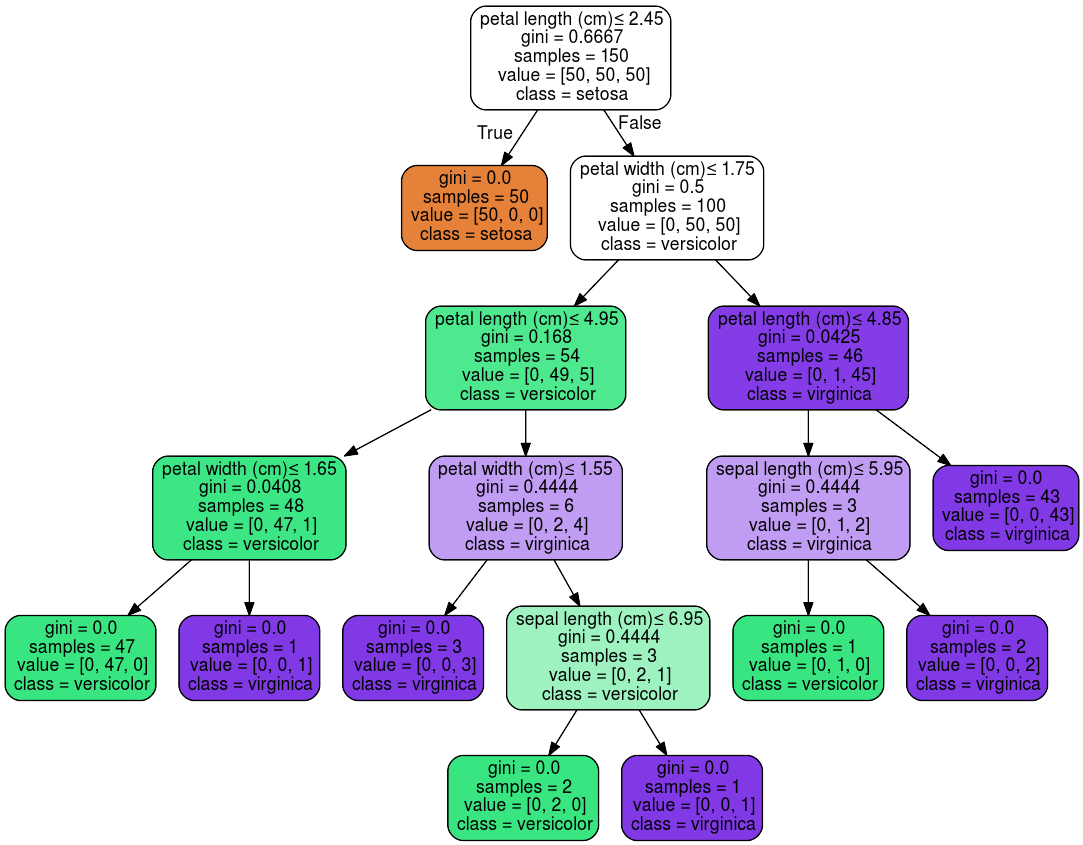
\includegraphics[scale=.4]{iris.png}
	\caption{Estructura de árbol para modelo de clasificación de set de datos iris.}
	\label{arboles}
\end{figure}


Un árbol puede ser entrenado mediante el fraccionamiento del conjunto inicial en subconjuntos basados en una prueba de valor de atributo. Este proceso se repite en cada subconjunto derivado de una manera recursiva, el cual es denominado \textit{particionamiento recursivo}. La recursividad termina cuando el subconjunto en un nodo $m$ tiene todos sus miembros el mismo valor de la variable categórica o pertenecen al mismo intervalo finito, para el caso en que las respuestas se asocian a distribuciones continuas, o cuando la partición ya no agrega valor a las predicciones.

Para cada división, es necesario el uso de una función que entregue una medida de impureza en cada partición, esto, con el objetivo de seleccionar el mejor subconjunto para un atributo dado, la elección de dicho descriptor, se basa en el objetivo de separar de mejor manera los ejemplos. 

La selección de los atributos se basa en qué atributo, al momento de clasificar, genera nodos más puros. Para ello, se utiliza una función de ganancia de información, la cual representa la ganancia  obtenida a partir de una división de los ejemplos de entrenamiento \cite{breiman2017classification}. 

Existen diferentes tipos de algoritmos bajo los cuales son implementados las ideologías de los árboles de decisión, cada uno presenta características particulares. Sin embargo, cumplen con el mismo objetivo. A modo general, en la Tabla \ref{tab:summary-alg-trees} se exponen algunos de los algoritmos existentes \cite{hssina2014comparative}.

% Please add the following required packages to your document preamble:
% \usepackage{longtable}
% Note: It may be necessary to compile the document several times to get a multi-page table to line up properly
\begin{longtable}[c]{|l|l|}
	\hline
	\multicolumn{2}{|c|}{\textbf{Algoritmos de árboles de decisión}} \\ \hline
	\endfirsthead
	%
	\endhead
	%
	\multicolumn{1}{|c|}{\textbf{Algoritmo}} & \multicolumn{1}{c|}{\textbf{Descripción}} \\ \hline
	Iterative Dichotomiser 3 (ID3) & \begin{tabular}[c]{@{}l@{}}Se crea un árbol de múltiples vías, encontrando para cada\\ nodo la característica categórica que producirá la mayor\\ ganancia de información. Por lo general, se aplica un\\ paso de poda para mejorar la capacidad del árbol asociada\\ a la generalización.\end{tabular} \\ \hline
	C4.5 & \begin{tabular}[c]{@{}l@{}}Permite manipular variables continuas, mediante la definición\\ dinámica de atributos discretos, dividiendo el valor continuo en\\ un conjunto finito de intervalos discretos. La poda se realiza\\ eliminando la condición previa de una regla si la precisión de\\ la regla mejora sin ella.\end{tabular} \\ \hline
	C5.0 & \begin{tabular}[c]{@{}l@{}}Genera un conjunto de reglas más pequeñas en comparación a\\ C4.5. Sin embargo, este último es más preciso en cuanto al \\ entrenamiento.\end{tabular} \\ \hline
	\begin{tabular}[c]{@{}l@{}}Classification and Regression\\ Trees (CART)\end{tabular} & \begin{tabular}[c]{@{}l@{}}Construye árboles binarios utilizando la característica y el\\ umbral que producen la mayor ganancia de información en\\ cada nodo.\end{tabular} \\ \hline
	\caption{Resumen de algoritmos comunes para la creación de árboles de decisión. }
	\label{tab:summary-alg-trees}\\
\end{longtable}

\subsubsection{Formulación matemática}

Una definición matemática, tanto del proceso de clasificación o regresión y cómo son los criterios de selección de atributos es expuesta a continuación.

Sea $x_{i} \in R^{n}$ los vectores de entrenamiento del conjunto de datos y sea $y \in R^l$ el vector de respuestas asociadas a cada ejemplo. Un árbol de decisión divide el espacio de forma recursiva, de manera que las muestras con las mismas etiquetas se agrupan.

Cada nodo $m$ puede ser representado por $Q$ y sea $\theta = (j, t_{m})$ la división candidata para un atributo $j$ y un umbral $t_{m}$, se definen las particiones $Q_{left}(\theta)$ y $Q_{rigth}(\theta)$ tal que:

\begin{align}
	\begin{aligned}
		Q_{left}(\theta) = {(x, y) | x_j <= t_m}\\Q_{right}(\theta) = Q \setminus Q_{left}(\theta)
	\end{aligned}
\end{align}
 

Asociado a las divisiones, se tiene que, cada nodo generado se mide con respecto a la impureza de éste, la cual, puede ser representada por una función $H()$ y a la ganancia de información que genera la división $G(Q, \theta)$, la cual se estima como:

\begin{center}
	$G(Q, \theta) = \frac{n_{left}}{N_m} H(Q_{left}(\theta))
+ \frac{n_{right}}{N_m} H(Q_{right}(\theta)$
\end{center}

Los descriptores se seleccionan con respecto a aquel que minimice la impureza de los nodos:

\begin{center}
	$\theta^* = \operatorname{argmin}_\theta  G(Q, \theta)$
\end{center}

Finalmente, se tiene que para los subconjuntos $Q_{left}(\theta^*)$ y $Q_{rigth}(\theta^*)$ la profundidad máxima se alcanza si:

\begin{itemize}
	
	\item $N_{m} < min_{samples}$ 
	
	\item $N_{m} = 1$
\end{itemize}

Con $N_{m}$ representando el número de nodos $m$.

Los criterios de clasificación se basan en la proporción de las clases según sus observaciones y en la función de impureza que es posible utilizar.

Si el vector de respuestas, es asociado a variables categóricas y toma valores entre $0,1,\cdots,k-1$ para un nodo $m$, representando una región $R_{m}$ con $N_{m}$ ejemplos, se tiene que la proporción  de observaciones de clase $k$ en un nodo $m$ puede definirse como:

\begin{center}
	$p_{mk} = 1/ N_m \sum_{x_i \in R_m} I(y_i = k)$
\end{center}

Con respecto a las diferentes funciones de impureza $H()$ que pueden ser utilizadas se tienen las siguientes, descritas en la Tabla \ref{tab:tab-form-impureza}. 

% Please add the following required packages to your document preamble:
% \usepackage{longtable}
% Note: It may be necessary to compile the document several times to get a multi-page table to line up properly
\begin{longtable}[c]{|l|l|}
	\hline
	\multicolumn{1}{|c|}{\textbf{Función}} & \multicolumn{1}{c|}{\textbf{Fórmula}}   \\ \hline
	\endfirsthead
	%
	\endhead
	%
	Gini                                   & $H(X_m) = \sum_k p_{mk} (1 - p_{mk})$   \\ \hline
	Entropía                               & $H(X_m) = - \sum_k p_{mk} \log(p_{mk})$ \\ \hline
	\textit{Misclassification}                      & $H(X_m) = 1 - \max(p_{mk})$             \\ \hline
	\caption{Tipos de medidas de impureza que pueden ser utilizadas en árboles de decisión para modelos de clasificación.
	}
	\label{tab:tab-form-impureza}\\
\end{longtable} 

Siendo $X_{m}$ datos de entrenamiento en el nodo $m$.

A la hora de entrenar modelos de regresión, es decir, con respuestas asociadas a una distribución continua, se tiene que para el nodo $m$, el cual representa una región $R_{m}$ con observaciones $N_{m}$, los criterios comunes para minimizar errores en futuras divisiones son el Error cuadrático medio y el Error absoluto medio, quienes minimizan el error tipo II y el error tipo I, respectivamente.

Estos se pueden definir como:

\begin{itemize}
	
	\item \textbf{Error cuadrático medio}: 
	
	\begin{align}\begin{aligned}\bar{y}_m = \frac{1}{N_m} \sum_{i \in N_m} y_i\\H(X_m) = \frac{1}{N_m} \sum_{i \in N_m} (y_i - \bar{y}_m)^2\end{aligned}\end{align}
	
	\item \textbf{Error absoluto medio}: 
	
	\begin{align}\begin{aligned}\bar{y}_m = \frac{1}{N_m} \sum_{i \in N_m} y_i\\H(X_m) = \frac{1}{N_m} \sum_{i \in N_m} |y_i - \bar{y}_m|\end{aligned}\end{align}
\end{itemize}

Este tipo de entrenamiento, es uno de los más utilizados, debido a su simplicidad a la forma en la que trabaja, ya que, permite comprender del problema, con respecto a los atributos y cómo estos van distribuyendo las respuestas, así, es posible entender las decisiones que toma el algoritmo para clasificar o predecir nuevos ejemplos, determinar comportamientos preferentes y tendencias sobre atributos y rangos de estos.

\subsection{Support Vector Machine (SVM)}

Máquina soporte de vectores (SVM por sus siglas en inglés), es un conjunto de métodos de aprendizaje supervisado, utilizados para clasificar, predecir e inclusive para la detección de puntos outliers  \cite{scholkopf2001learning}. 

SVM genera una representación de los ejemplos como puntos en el espacio, mapeados de modo que los ejemplos de las categorías separadas se dividan por un espacio claro que es tan amplio como sea posible. Nuevos ejemplos son entonces mapeados en ese mismo espacio y predicen si pertenecen a una categoría en base a qué lado del espacio son asignados \cite{scholkopf2001learning}.

Las predicciones se realizan de manera eficiente, utilizando funciones kernel para su transformación en espacios no lineales \cite{amari1999improving}. Esto permite generar transformaciones de espacio dimensional de los datos, para mapear implícitamente sus entradas en espacios característicos de alta dimensión. 

Las funciones de kernel que pueden ser utilizadas, son descritas en la Tabla \ref{tab:tab-kernel}

% Please add the following required packages to your document preamble:
% \usepackage{longtable}
% Note: It may be necessary to compile the document several times to get a multi-page table to line up properly
\begin{longtable}[c]{|l|l|}
	\hline
	\multicolumn{1}{|c|}{\textbf{Kernel}} & \multicolumn{1}{c|}{\textbf{Fórmula}}   \\ \hline
	\endfirsthead
	%
	\endhead
	%
	Lineal                                & $\langle x, x'\rangle$                  \\ \hline
	Polinomial                            & $(\gamma \langle x, x'\rangle + r)^d$   \\ \hline
	Radio basis function (RBF)            & $\exp(-\gamma \|x-x'\|^2)$              \\ \hline
	Sigmoideo                             & $\tanh(\gamma \langle x,x'\rangle + r)$ \\ \hline
	\caption{Tipos de kernels aplicados por SVM para la transformación espacial de los datos.
	}
	\label{tab:tab-kernel}\\
\end{longtable}

Existen ventajas y desventajas al usar SVM como algoritmo de aprendizaje supervisado, las cuales se listan a continuación.

\begin{itemize}
	
	\item Efectivo en espacios de alta dimensión.
	\item Eficiente cuando el número de atributos supera a la cantidad de ejemplos en un conjunto de datos.
	\item Utiliza un subconjunto de puntos de entrenamiento en la función de decisión (llamada
	vectores de soporte), por lo que también es memoria eficiente.
	\item Versátil: diferentes funciones de kernel pueden ser especificadas para la función de decisión. 
	
\end{itemize}

Las desventajas de las máquinas de soporte vectorial incluyen:

\begin{itemize}
	
	\item Si el número de características es mucho mayor que el número de muestras, es probable que
	el método tenga un mal desempeño.
	\item SVM no proporciona directamente estimaciones de probabilidad \cite{wu2004probability}, estos se calculan utilizando cinco veces una costosa validación cruzada.
	
\end{itemize}

Existen diversas variaciones de SVM, tales como: SVC \cite{guyon1993automatic}, $\nu$SVC y LinearSVC, los cuales son capaces de realizar una clasificación multiclase\footnote{Implica la existencia de un número de clases mayor a dos} en un conjunto de datos, es decir, ya no depender de un clasificador binario. A su vez, presentan sus variantes para el entrenamiento de modelos de regresión, asociados a respuestas con distribución continua, denominados SVR, $\nu$SVR y LinearSVR, respectivamente.

De manera simple, se puede describir algunos puntos como:

\begin{itemize}

	\item SVC es implementado basado en libsvm \cite{chang2011libsvm}. La complejidad del tiempo de ajuste se hace cuadrática con el número de muestras, lo que dificulta escalar a conjunto de datos con tamaño mayor a 10000 ejemplos.

	\item Por otro lado, $\nu$SVC presenta características similares a SVC. Pero, utiliza el parámetro $\nu$ para controlar el número de vectores de soporte. Su implementación, al igual que SVC se basa en libsvm.

	\item LinearSVC es similar a SVC pero, se utiliza una función de kernel lineal. Además, es implementado en términos de liblinear, por lo que tiene más flexibilidad en la elección de las penalizaciones y las funciones de pérdida y facilita una mayor escalabilidad para conjuntos de datos con gran cantidad de ejemplos.
	
\end{itemize}


Cada uno de los clasificadores expuestos en los puntos anteriores toman como entrada el set de entramiento y las etiquetas asociadas a las clases, con el fin de generar tanto el testeo como la validación del modelo.

Previo a la etapa de entrenamiento, se utilizan vectores de apoyo para el set de entrenamiento, los que son denominados vectores de soporte, normalmente obtenidos a partir de funciones de kernel para.

SVC y NuSVC implementan el enfoque \textit{uno contra uno} para la clasificación multiclase. Si existen $n$ clases, se construyen $\frac{n*(n-1)}{2}$ clasificadores, de los cuales cada uno forma un set datos de dos clases; por otro lado, LinearSVC implementa una estrategia multi-clase \textit{uno contra el resto}, formando así modelos de $n$ clases, los cuales son entrenados $n$ veces. Si sólo hay dos clases, sólo se entrena un modelo.

Los algoritmos SVM están asociados a diversos problemas. Sin embargo, el principal, radica en el desbalance de clases, ya sea por el número que presentan o por el peso asociado a éstas, tal como se expone en la Figura  \ref{SVM1}:

\begin{figure}[!h]
	
	\centering
	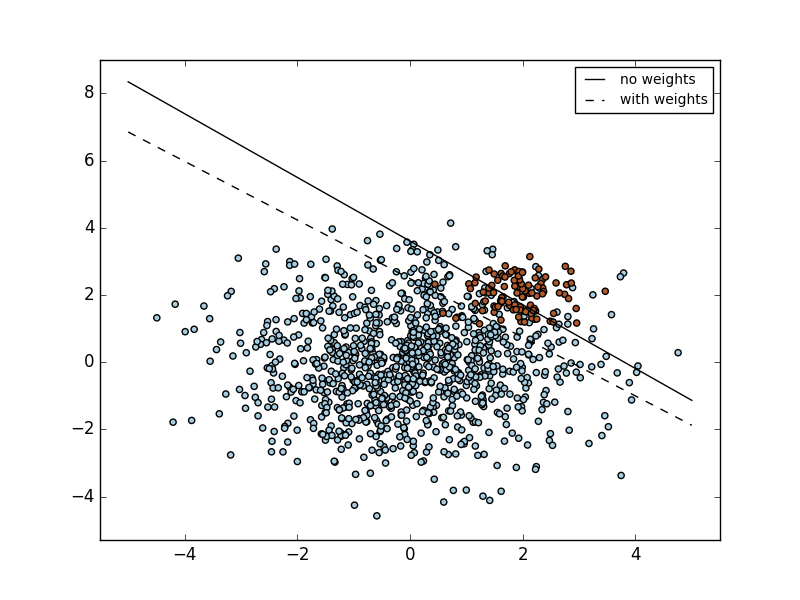
\includegraphics[scale=.5]{SVM1.png}
	\caption{Muestra de desbalance de clases en SVM.}
	\label{SVM1}
\end{figure}

\subsubsection{Formulación matemática}

SVM construye un hiperplano o un conjunto de hiperplanos en un espacio altamente dimensiona, el cual es utilizado tanto para la clasificación de elementos, com para la predicción de valores continuos, a su vez, puede ser implementado para detección de puntos outliers. 

Intuitivamente, se logra una buena separación por el hiper plano que tiene la mayor distancia a los puntos de datos de entrenamiento más cercanos de cualquier clase, ya que en general, cuanto mayor sea la separación, menor será el error de generalización del modelo.

Es posible observar este comportamiento en la Figura \ref{SVM2}

\begin{figure}[!h]
	\centering
	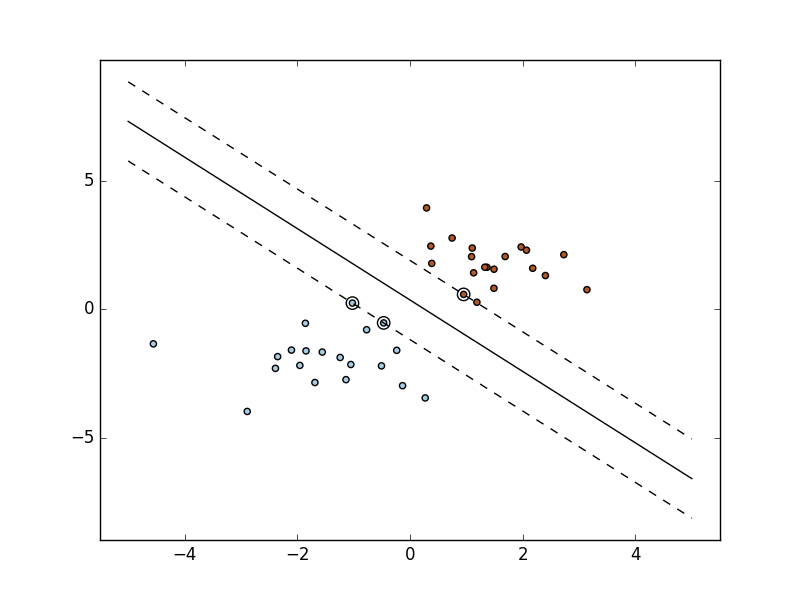
\includegraphics[scale=.5]{SVM2.png}
	\caption{Esquema de hiperplanos en SVM.}
	\label{SVM2}
	
\end{figure}

Es posible entregar una definición matemática para SVM, haciendo una diferenciación asociados a los métodos de clasificación y regresión. De tal manera que, para SVC, se tiene que:

Dado los vectores de entrenamiento $x_{i}\ \in\ R$,
i=1,..., n, en dos clases, y un vector, $y \in \{1, -1\}^n$, SVC resuelve el siguiente problema primario:

\begin{center}
	$\min_ {w, b, \zeta} \frac{1}{2} w^T w + C \sum_{i=1}^{n} \zeta_i$
\end{center}
\begin{center}
	
	$para\ la\ clase\ y_i (w^T \phi (x_i) + b) \geq 1 - \zeta_i,\ \zeta_i \geq 0, i=1, ..., n$	
\end{center}

Su doble es

\begin{center}
	$\min_{\alpha} \frac{1}{2} \alpha^T Q \alpha - e^T \alpha$
\end{center}
\begin{center}
	$para\ la\ clase\ y^T \alpha = 0\ 0 \leq \alpha_i \leq C, i=1, ..., n$
\end{center}

Donde $e$ es el vector de todos los unos, $C > 0$ es el límite superior, $Q$ es una matriz de $n\ x\ n$ definida semipositiva, $Q_{ij} \equiv y_i y_j K(x_i, x_j)$, donde $K(x_i, x_j) = \phi (x_i)^T \phi (x_j)$ es el kernel. Los vectores de entrenamiento son implícitamente mapeados en un espacio dimensional mayor (tal vez infinito) por la función $\phi$.

La función de decisión es:

\begin{center}
	$sgn(\sum_{i=1}^n y_i \alpha_i K(x_i, x) + \rho)$
\end{center}

Por otro lado, $\nu$SVC presenta características similares a SVC. No obstante, el uso del parámetro $\nu$ permite controlar el número de vectores de soporte y errores de entrenamiento. $\nu \in (0, 1]$ y  es un límite superior en la fracción de errores de entrenamiento y un límite inferior de la fracción de vectores de soporte.

A su vez, LinearSVC presenta el mismo comportamiento a SVC. Sin embargo, la gran diferencia es la utilización de un kernel lineal como función de transformación de espacio y evaluación de puntos.

Finalmente, ya que SVM también permite entrenar modelos de regresión particularmente con SVR, una definición matemática de éste se expone como:

Dados los vectores de entrenamiento  $x_{i} \in\ R^n$  
$\varepsilon-SVR$ \cite{smola2004tutorial} resuelve el siguiente problema primario:

\begin{center}
	
	$\min_ {w, b, \zeta, \zeta^*} \frac{1}{2} w^T w + C \sum_{i=1}^{n} (\zeta_i + \zeta_i^*)
	$
\end{center}

\begin{center}
	
	$para\ la\ clase\ y_i - w^T \phi (x_i) - b \leq \varepsilon + \zeta_i,$
\end{center}
\begin{center}
	$w^T \phi (x_i) + b - y_i \leq \varepsilon + \zeta_i^*,\ \zeta_i, \zeta_i^* \geq 0, i=1, ..., n$	
\end{center}

Donde $e$ es el vector para todos, $C >$ 0 es el límite superior, $Q$ es una matriz de $n\ x\ n$ definida semipositiva, $Q_{ij} \equiv K(x_i, x_j) = \phi (x_i)^T \phi (x_j)$ es el kernel. Aquí los vectores de
entrenamiento son implícitamente mapeados en un espacio dimensional mayor (tal vez infinito) por
la función $\phi$.

La función de decisión es:

\begin{center}
	$\sum_{i=1}^n (\alpha_i - \alpha_i^*) K(x_i, x) + \rho$
\end{center}

Como se puede observar, las formulaciones matemáticas, tanto para SVC como SVR son similares. Sin embargo, se diferencian en la función de decisión a utilizar, esto es debido a que SVC es un clasificador, mientras que SVR es un métodos de regresión.

\subsection{Métodos de ensamble}

Los métodos de ensamble, se basan en la combinación de las predicciones obtenidas por varios estimadores, construidos en base a algoritmos de aprendizaje supervisado, con el fin de mejorar la generalización del modelo y aumentar la robustez ante nuevos ejemplos \cite{dietterich2000ensemble}.

Existen dos familias de métodos de ensamble, las cuales se diferencian principalmente en la forma en que combinan los modelos para obtener la medida de desempeño final \cite{kotsiantis2007supervised}:

\begin{enumerate}
	
	\item \textbf{Métodos ponderados}: basados en la construcción de varios estimadores independientes y promediar sus medidas de desempeño, esto mejora el rendimiento debido a que disminuye la variabilidad de las clasificaciones. Ejemplos comunes de esto son Bagging y Random Forest.
	
	\item \textbf{Métodos boosting}: basados en la construcción secuencial de modelos, intentando disminuir el sesgo del modelo combinando diferentes estimadores débiles. Cumple con la filosofía \textit{"la unión de varios modelos débiles, puede construir uno fuerte"}. Ejemplos comunes de esto son AdaBoost y Gradient Tree Boosting.
	
\end{enumerate}

A continuación, se explican brevemente algunos de los algoritmos asociados a la familia de métodos de ensamble.

\subsubsection{Bagging}

Bagging forma parte de los métodos ponderados, en particular, se puede definir como métodos que forman una clase de algoritmos compuestos por varias instancias de un estimador, entrenados en base a subconjuntos aleatorios del set de datos original, ponderando sus predicciones individuales en una respuesta ponderada. El objetivo general de estos métodos es reducir la varianza de un estimador, por medio del proceso de entrenamiento de subconjuntos aleatorios \cite{breiman1996bagging}. 

Existen diferentes formas de generar los subconjuntos aleatorios de entrenamiento, dentro de las cuales se destacan las siguientes.

\begin{itemize}
	
	\item Los subconjuntos aleatorios del conjunto de datos se basan en subconjuntos aleatorios de las muestras, esto se conoce como \textit{"Pasting o Pegado"} \cite{breiman1999pasting}. 
	
	\item Las muestras se extraen con reemplazo, siendo este método conocido como \textit{"Bagging"} \cite{breiman1996bagging}.
	
	\item Los subconjuntos aleatorios del conjunto de datos se basan en subconjuntos aleatorios de las características, esto se conoce como \textit{"subespacios aleatorios"} \cite{barandiaran1998random}.
	
	\item Los subconjuntos aleatorios se crean en base a subconjuntos aleatorios de características y muestras, esto se conoce como \textit{"Random Patches"} \cite{ref10.1007/978-3-642-33460-3_28}.
	
\end{itemize}

\subsubsection{Random Forest \label{rf}}

Random Forest es un método de ensamble ponderado basado en árboles de decisión aleatorios. Conjuntos de diversos clasificadores son creados basados en efectos aleatorios tanto de la extracción de características como de ejemplos, formando subconjuntos de elementos, cada uno de estos aporta con un valor de estimación, el cual es ponderado con los restantes, obteniendo así, la medida general \cite{breiman1998}.

Un esquema representativo del proceso, es como se expone en la Figura \ref{rf1}. En ella, se aprecian que se generan $n$ árboles, los cuales contemplan diferentes cantidades de ejemplos o atributos y la estimación final se basa en una ponderación, ya sea por proceso de votación, en el caso de modelos de clasificación, o simplemente por la media, para modelos de regresión \cite{Breiman2001}.

\begin{figure}[!h]
	\centering
	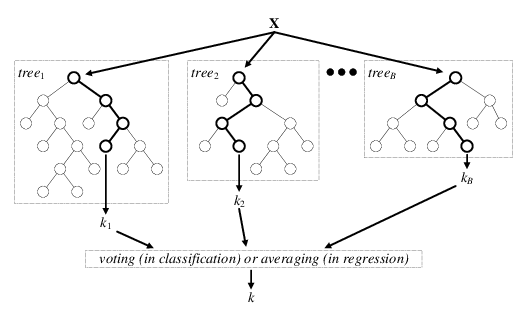
\includegraphics[scale=.5]{rf.png}
	\caption{Esquema representativo de algoritmo Random Forest.}
	\label{rf1}
	
\end{figure}

\subsubsection{AdaBoost}

AdaBoost, es un algoritmo basado en el método boosting, lo que implica que se ajusta a una secuencia de estimadores débiles obtenidos a partir de diferentes subconjuntos de datos generados de manera aleatoria desde el conjunto inicial de datos de entrenamiento \cite{CAO2013745}. 

Cada una de las predicciones obtenidas por los estimadores se combinan de manera ponderada por votación, en el caso de modelos de clasificación, o a través de un promedio en base a las estimaciones resultantes, en el caso de modelos de regresión.

Las modificaciones de los datos en cada iteración de boosting, consisten en aplicar pesos $w_{1},w_{2},..,w_{N}$, a cada una de las muestras de entrenamiento. 

Inicialmente, todos los pesos están configurados en $\Psi_{i}\ =\ 1/N$, de modo que el primer paso simplemente entrena un modelo débil en los datos originales. Para cada iteración sucesiva, las ponderaciones de la muestra se modifican individualmente y el algoritmo de aprendizaje se vuelve a aplicar a los datos ponderados. 

En un paso dado, los ejemplos de entrenamiento que fueron predichos incorrectamente por el modelo mejorado inducido en el paso anterior tienen sus pesos incrementados, mientras que los pesos se disminuyen para aquellos que fueron predichos correctamente \cite{hastie2009multi}. 

A medida que avanzan las iteraciones, los ejemplos que son difíciles de predecir reciben una influencia cada vez mayor. Por lo tanto, cada modelo de aprendizaje débil subsiguiente se ve forzado a concentrarse en los ejemplos que se pierden en los anteriores en la secuencia.

\subsubsection{Gradient Tree Boosting}

Gradient Tree Boosting o Gradient Boosted Regression Trees, es una generalización de métodos de boosting para funciones diferenciables arbitrarias de pérdida \cite{gradient}. Es un método considerado como preciso y efectivo, el cual puede usarse tanto para el desarrollo de modelos de clasificación como de regresión, siendo usado en diferentes áreas de investigación: motores de búsqueda, ecología, minerología, biotecnología, entre otros.

Dentro de las principales ventajas que posee, se encuentran: manejo natural de diferentes tipos de características en un set de datos, alto poder predictivo y robusto frente a la predicción de valores atípicos en una muestra \cite{FRIEDMAN2002367}.

Como formulación matemática, se tiene, la adición de modelos se basa en:

\begin{center}
	$F(x) = \sum_{m=1}^{M} \gamma_m h_m(x)$
\end{center}

Donde $h_{m}(x)$ es una función básica, conocida como \textit{weak learners} en el contexto de boosting. En particular, Gradient Tree Boosting, utiliza árboles de decisión de tamaño fijo como \textit{weak learners}. 


Los modelos aditivos, se construyen de manera incremental, tal que:

\begin{center}
	$F_m(x) = F_{m-1}(x) + \gamma_m h_m(x)$
\end{center}

De tal manera que el nuevo árbol agregado $h_{m}$ trata de minimizar la pérdida $L$ dado el previo ensamble $F_{m-1}$, es decir:

\begin{center}
	$h_m =  \arg\min_{h} \sum_{i=1}^{n} L(y_i, F_{m-1}(x_i) + h(x_i))$
\end{center}

Este algoritmo, resuelve el problema de minimización numéricamente, a través de steepest descent \cite{battiti1992first}. La dirección de steepest descent es el gradiente negativo de la función de pérdida $L$ evaluada en el modelo actual $F_{m-1}$, el cual puede ser calculado para cualquier función de pérdida diferenciable, tal que:

\begin{center}
	$F_m(x) = F_{m-1}(x) - \gamma_m \sum_{i=1}^{n} \nabla_F L(y_i, F_{m-1}(x_i))$
\end{center}

Donde la longitud del paso $\gamma_{m}$ es seleccionada mediante una búsqueda lineal, aplicando:

\begin{center}
	$\gamma_m = \arg\min_{\gamma} \sum_{i=1}^{n} L(y_i, F_{m-1}(x_i) - \gamma \frac{\partial L(y_i, F_{m-1}(x_i))}{\partial F_{m-1}(x_i)})$
\end{center}

A la hora de estimar un valor continuo por medio de algoritmos de regresión o clasificar un nuevo ejemplo a través de un clasificador, existe una única diferencia, la cual radica en la función de pérdida $L$ que es utilizada. En la Tabla \ref{tab:function-loss} se resumen las funciones de pérdida y sus definiciones, normalmente utilizadas en métodos basados en Gradient Tree Boosting.

% Please add the following required packages to your document preamble:
% \usepackage{longtable}
% Note: It may be necessary to compile the document several times to get a multi-page table to line up properly
\begin{longtable}[c]{|l|l|l|}
	\hline
	\multicolumn{3}{|c|}{\textbf{Funciones de pérdida utilizadas en métodos GTB}} \\ \hline
	\endfirsthead
	%
	\endhead
	%
	\multicolumn{1}{|c|}{\textbf{Función}} & \multicolumn{1}{c|}{\textbf{Descripción}} & \multicolumn{1}{c|}{\textbf{Uso}} \\ \hline
	Least squares & \begin{tabular}[c]{@{}l@{}}Valor inicial se obtiene a partir de la\\ media de los vectores respuesta\end{tabular} & Regresión \\ \hline
	Least absolute deviation & \begin{tabular}[c]{@{}l@{}}Valor inicial se obtiene a partir de la\\ mediana de los vectores respuesta\end{tabular} & Regresión \\ \hline
	Huber & \begin{tabular}[c]{@{}l@{}}Combina el uso de mínimos cuadrados\\ y los errores absolutos\end{tabular} & Regresión \\ \hline
	Quantile & \begin{tabular}[c]{@{}l@{}}Se basa en el uso de cuantiles para\\ crear rangos de predicción\end{tabular} & Regresión \\ \hline
	Binomial deviance & \begin{tabular}[c]{@{}l@{}}Se basa en la distribución de probabilidad\\ binomial, para modelos binarios de\\ clasificación\end{tabular} & Clasificación \\ \hline
	Multinomial deviance & \begin{tabular}[c]{@{}l@{}}Se basa en la distribución de probabilidad\\ multinomial y su valor inicial corresponde\\ a las probabilidades a priori de cada\\ categoría\end{tabular} & Clasificación \\ \hline
	Exponential loss & \begin{tabular}[c]{@{}l@{}}Se basa en distribución exponencial y sólo\\ puede ser utilizada en modelos de clasificación\\ binarios\end{tabular} & Clasificación \\ \hline
	\caption{Funciones de pérdida comunes utilizadas en los algoritmos Gradient Tree Boosting, ya sea en forma de clasificador como regresor.}
	\label{tab:function-loss}\\
\end{longtable}

\subsection{Redes Neuronales y Deep Learning}

Redes neuronales es posible definirlas como una serie de modelos de aprendizaje que se basan en la forma de trabajo de las redes neuronales biológicas, es decir, se usa el concepto de \textit{neurona} para estimar una función aproximada, la cual dependerá de un largo número de inputs, generalmente desconocidos.

En la Figura \ref{red} se aprecia un sistema de red neuronal, en la cual se observa un sistema interconectado por neuronas, las cuales intercambian información en forma de mensaje entre ellas, además cada interconexión tiene un peso, el cual es un valor numérico, que puede ser obtenido en base a la experiencia.

En resumen, una red neuronal es un conjunto de entradas y salidas regidas por capas intermedias que permiten evaluar la salida, dichas capas operan entre sí en base a funciones matemáticas y brindan un peso a la conexión, finalmente cada capa es usada para diseñar un modelo de aprendizaje supervisado o no.

\begin{figure}[!h]
	\centering
	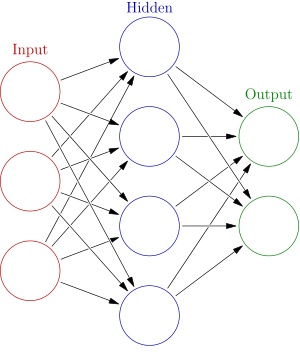
\includegraphics[scale=.5]{red.png}
	\caption{Representación esquemática de una Red Neuronal}
	\label{red}
\end{figure} 

Deep Learning es una herramienta de Machine Learning la cual tiene por objetivo modelar abstracciones de alto nivel en los datos por medio del uso de múltiples capas de procesamiento, ya sea a través del uso de estructuras complejas a través de múltiples transformaciones no lineales \cite{bengio2013representation, MAL-006, SIG-039}. 

La investigación en esta área tiene por objetivo generar mejores representaciones y crear modelos para aprender de éstas a partir de datos no marcados a gran escala. En geneal, las representaciones obtenidas se inspiran en los avances en la neurociencia y se basa libremente en la interpretación de los patrones de procesamiento y comunicación de información en un sistema nervioso, como la codificación neural que intenta definir una relación entre varios estímulos y respuestas neuronales asociadas en el cerebro \cite{MAL-006}.

Deep learning es un método específico de machine learning el cual incorpora redes neuronales organizadas en capas consecutivas para poder aprender iterativamente utilizando un conjunto de datos. Deep learning es especialmente útil cuando se desea aprender patrones provenientes de datos no estructurados \cite{SIG-039}.

Posee diversas arquitecturas, tales como: deep learning network, matrices de convoluciones, redes neuronales recurrentes, etc. las cuales han sido utilizadas en visión artificial para el reconocimiento de patrones, aprendizaje de escritura, etc. Deep Learning es una herramienta de Machine Learning la cual tiene por objetivo modelar abstracciones alto nivel en los datos por medio del uso de múltiples capas de procesamiento, ya sea a través del uso de estructuras complejas a través de múltiples transformaciones no lineales \cite{arel2010deep}.

Dentro de los principales algoritmos que son utilizados en redes neuronales se encuentran Back Propagation \cite{HECHTNIELSEN199265} y Multi Layer Perceptron \cite{80266}.

Si bien en la actualidad, redes neuronales y Deep Learning son metodologías ampliamente utilizadas y han tenido resultados satisfactorios a la hora de trabajar en diferentes áreas de investigación, presentan un problema relevante al momento de aprender de los datos, los atributos y cómo estos facilitan o distribuyen la información.

Este problema es debido a que, los sistemas de redes neuronales trabajan en torno a información oculta, denominados, sistemas de cajas negras, lo cual, no permite comprender cómo se genera una nueva clasificación o predicción de elementos. 

Lo anterior, no ocurre con métodos basados en estimaciones de distancia como KNN, uso de hiperplanos y funciones de kernel para la transformación espacial de los atributos como SVM, reglas de decisión que permiten representar estructuras de árbol que facilitan la comprensión de cómo distribuyen los atributos, rangos preferibles etc., como lo hacen los algoritmos basados en árboles de decisión e inclusive los métodos de ensamble. Es decir, diferentes algoritmos vislumbran cómo manipulan la información para llegar al resultado, no siendo el caso de las redes neuronales. Por lo tanto, dado a que se requiere de algoritmos que permitan la comprensión del problema y que posibiliten generar aprendizaje de los atributos, se descartan a priori el uso de métodos basados en redes neuronales y el uso de Deep Learning.


\subsection{Medidas de desempeño \label{desempeno}}

Medir el desempeño del modelo predictivo es importante a la hora de evaluar qué tan efectivo es el entrenamiento o la clasificación que se genera, existen medidas que sólo se basan en la cantidad de aciertos o errores que comete el clasificador, otras que implican la eficiencia del modelo y otras que se basan en la precisión.

A continuación, se define brevemente algunas de las medidas más utilizadas a la hora de evaluar modelos de aprendizaje supervisados:

\begin{itemize}
	
	\item \textbf{Tasa de Verdaderos Positivos}: corresponde a la medida asociada a las correctas clasificaciones versus el total de clasificaciones realizadas, es decir, cuántas predicciones efectivas se obtuvieron con respecto a una clase.
	
	\item \textbf{Tasa de Falsos Positivos}: corresponde a la medida asociada a las clasificaciones mal efectuadas, es decir, cuántas predicciones erradas existen con respecto a una clase.
	
	
	\item \textbf{Accuracy}: corresponde al total de predicciones correctas con respecto al total de la muestra. Sea $\hat{y}_i$ el valor de predicción del ejemplo $i$ e $y_{i}$ corresponde al verdadero valor, la Accuracy se define como: $\texttt{accuracy}(y, \hat{y}) = \frac{1}{n_\text{samples}} \sum_{i=0}^{n_\text{samples}-1} 1(\hat{y}_i = y_i)$
	
	\item \textbf{Precision}: es la capacidad del clasificador asociada a no etiquetar como positiva una muestra que es negativa, se define como: $\text{precision} = \frac{tp}{tp + fp}$, donde tp corresponde a verdaderos positivos y fp a los falsos positivos.
	
	
	\item \textbf{Recall}: es la capacidad del clasificador asociada encontrar todas las muestras positivas, se define como: $\text{recall} = \frac{tp}{tp + fn}$ , donde tp corresponde a verdaderos positivos y fp a los falsos positivos.
	
	\item \textbf{F-$\beta$}: representa una ponderación armónica entre la Precision y el Recall, se define como: $F_\beta = (1 + \beta^2) \frac{\text{precision} \times \text{recall}}{\beta^2 \text{precision} + \text{recall}}.$ , donde $\beta$ un factor de ponderación.
	
	\item \textbf{Coeficiente de correlación de Matthews}: Se asocia a una medida de la calidad de las clasificaciones, la cual no se ve afectada por el desbalance de clases que pudiese existir, se define como $MCC = \frac{tp \times tn - fp \times fn}{\sqrt{(tp + fp)(tp + fn)(tn + fp)(tn + fn)}}$, donde tp corresponde a verdaderos positivos y fp a los falsos positivos.
	
\end{itemize}
	
Las mediciones expuestas previamente, se utilizan para medir el desempeño de modelos de clasificación, mientras que para evaluar un estimador basado en respuestas continuas, normalmente se utilizan las siguientes:
	
\begin{itemize}
		
	\item \textbf{Coeficiente de Pearson}: Medida lineal entre dos variables cuantitativas aleatorias que permite evaluar el grado de relación entre ellas, se encuentra en rangos entre -1 y 1 donde -1 indica que las variables no presentan relación y 1 que las muestras están estrechamente relacionadas. Se obtiene a partir de $\rho X,Y= \frac{n\sum x_{i}y_{i} - \sum x_{i} \sum y_{i}}{\sqrt{n\sum x^{2}_{i}- (\sum x_{i})^{2}} \sqrt{n\sum y^{2}_{i}- (\sum y_{i})^{2}}}$ donde $x_{i}$ representa los valores de predicción e $y_{i}$ representa los valores reales de la muestra para $n$ ejemplos.
		
	\item \textbf{Coeficiente de Spearman}: Medida de correlación que permite evaluar la asociación o relación entre dos muestras, su interpretación es similar al coeficiente de Pearson y se estima a partir de $\rho = 1- \frac{6\sum D^{2}}{N(N^{2}-1)}$ donde $D$ es la diferencia $x-y$ para el $i-th$ ejemplo y $N$ es el total de ejemplos en la muestra.
		
	\item \textbf{Kendall $\tau$ rank}: Medida que permite evaluar la relación entre dos variables, su interpretación es similar a las basadas en coeficiente de Pearson y Spearman. Se obtiene a partir de $\tau = \frac{\text{(numbers of concordant pairs)} - \text{(number of discordant pairs)}}{n(n-1)/2}$
		
	\item \textbf{Coeficiente de determinación $R^{2}\ score$}: es una medida que cuantifica cómo el predictor se adapta a nuevos ejemplos, posee un rango entre -1 y 1 donde -1 es lo peor y 1 lo mejor, esto es debido a que el estimador puede bajar su rendimiento. Se estima en base a $R^2(y, \hat{y}) = 1 - \frac{\sum_{i=0}^{n_{\text{samples}} - 1} (y_i - \hat{y}_i)^2}{\sum_{i=0}^{n_\text{samples} - 1} (y_i - \bar{y})^2}$ donde $\hat{y}_i$ corresponde al valor predicho para el $i-th$ ejemplo e $y_{i}$ corresponde al valor real en una muestra de $n-samples$.
		
	\item \textbf{Error medio absoluto}: Estima la diferencia positiva entre el valor real y el valor predicho para un conjunto de ejemplos. Se estima a partir de $\text{MAE}(y, \hat{y}) = \frac{1}{n_{\text{samples}}} \sum_{i=0}^{n_{\text{samples}}-1} \left| y_i - \hat{y}_i \right|.$ donde $\hat{y}_i$ corresponde al valor predicho para el $i-th$ ejemplo e $y_{i}$ corresponde al valor real en una muestra de $n-samples$.
		
	\item \textbf{Error cuadrático medio}: Estima la diferencia cuadrática entre el valor real y el valor predicho para un conjunto de ejemplos. Se obtiene a partir de $\text{MSE}(y, \hat{y}) = \frac{1}{n_\text{samples}} \sum_{i=0}^{n_\text{samples} - 1} (y_i - \hat{y}_i)^2$ donde $\hat{y}_i$ corresponde al valor predicho para el $i-th$ ejemplo e $y_{i}$ corresponde al valor real en una muestra de $n-samples$.
		
	\item \textbf{Error logarítmico cuadrático medio}: Es similar al error cuadrático medio, la diferencia principal es que se utiliza el logaritmo natural de las diferencias entre respuesta y valor predicho. Se estima en base a $\text{MSLE}(y, \hat{y}) = \frac{1}{n_\text{samples}} \sum_{i=0}^{n_\text{samples} - 1} (\log_e (1 + y_i) - \log_e (1 + \hat{y}_i) )^2$ donde $\hat{y}_i$ corresponde al valor predicho para el $i-th$ ejemplo e $y_{i}$ corresponde al valor real en una muestra de $n-samples$.
		
	\item \textbf{Error mediano absoluto}: es una medida robusta ante outliers, la pérdida o el error se calcula a partir de las medianas de las diferencias absolutas entre la respuesta y el valor predicho. Se estima en base a $\text{MedAE}(y, \hat{y}) = \text{median}(\mid y_1 - \hat{y}_1 \mid, \ldots, \mid y_n - \hat{y}_n \mid)$ donde $\hat{y}_i$ corresponde al valor predicho para el $i-th$ ejemplo e $y_{i}$ corresponde al valor real en una muestra de $n-samples$.
		
		
\end{itemize}

\subsection{Problemas asociados a los modelos de aprendizaje supervisado \label{problemas}}

Dentro de los principales problemas que pueden presentar los modelos de aprendizaje supervisado, se encuentran las situaciones en las que la cantidad de atributos que puede contener un set de datos es mucho mayor con respecto a la cantidad de ejemplos que se posee, conocido también como \textit{"Maldición de la dimensionalidad"} \cite{indyk1998approximate}.

Es posible definirla como: dado un conjunto de datos $nxm$ con $n$ ejemplos y $m$ descriptores, si $m >> n$, es decir, si $m= n\ x\ n$, es posible que ocurra dicha problemática.

Posibles soluciones a este problema comprenden técnicas asociadas a reducción de dimensionalidad \cite{sarwar2000application, van2009dimensionality}, siendo las más utilizadas \footnote{Estas técnicas, se explican en el capítulo \ref{cap3}}:

\begin{itemize}
	
	\item Métodos lineales de reducción como Análisis de componentes principales (PCA) y derivados.
	\item Análisis de características basados en modelos de clasificación/regresión aplicando Random Forest.
	\item Técnicas probabilísticas asociadas al Mutual Information.
	\item Evaluación de características relacionadas mediante coeficientes de Pearson o matrices de Correlación
\end{itemize}
 
En forma similar, también es posible que un set de datos contemple una gran cantidad de ejemplos y sus descriptores sean escasos. Estos casos se tratan con técnicas de reducción de dimensionalidad y contemplan la eliminación de ejemplos redundantes con el fin de maximizar la variabilidad de los ejemplos, técnicas como Mutual Information, Análisis de Correlaciones son bastante utilizadas en este problema.

Otro posible problema que se puede denotar es el sobreajuste \cite{hawkins2004problem}, esto quiere decir, que el modelo es extremadamente complejo, por lo que éste se ajusta muy bien al set de entrenamiento. No obstante, a la hora de probar con nuevos set de datos no representa la performance obtenida. 

Finalmente, un problema adicional a los modelos de clasificación se basa en el desbalance de clases \cite{japkowicz2002class}. Esto quiere decir, que existe una diferencia significativa entre los contadores de categorías asociadas a las clases, lo cual afecta a los algoritmos a la hora de entrenar, debido a que aumenta el riesgo de cometer errores del tipo I (falsos positivos). Normalmente, esto conlleva a una reducción de ejemplos de la clase mayoritaria en la etapa de entrenamiento o si es posible, la adición de nuevos ejemplos de la clase minoritaria. 

\subsection{Validación de modelos}

La validación de los modelos trata los problemas de sobreajuste y la generalización, es decir, evitar desarrollar modelos que sólo tengan buenas métricas o medidas de desempeño para los datos de entrenamiento y no permitan clasificar nuevos ejemplos. 

Con el fin de poder evitar esta problemática, normalmente los set de datos se dividen en 3 conjuntos: Entrenamiento, validación y testeo. Esto quiere decir, se considera una porción de elementos para entrenar el modelo, una segunda instancia para obtener las medidas de desempeño y una tercera con el fin de determinar si el clasificador entrega resultados acorde a las respuestas conocidas \cite{kohavi1995study}.

Existen técnicas que a partir del set de entrenamiento, generan múltiples divisiones, con el fin de entrenar subconjuntos de elementos del conjunto de entrenamiento y así obtener modelos ponderados.

La subdivisión en $n$ modelos para entrenar y generar modelos ponderados, permite aumentar la generalización del modelo, debido a que las medidas de desempeño varían levemente de aplicación en aplicación y al considerar las divisiones, se tienen distribuciones de las medidas del modelo. Dada las distribuciones, el entrenamiento reporta, la media de dicha distribución \cite{golub1979generalized}. 

Dentro de las principales técnicas de validación se encuentra la Validación cruzada con $k$ divisiones \cite{golub1979generalized} y un caso particular conocido como \textit{Leave one out}, en el cual el valor de $k$ es igual a la cantidad de ejemplos en el entrenamiento \cite{vehtari2017practical}. Éstas se explican a continuación.

\subsubsection{Validación Cruzada}

La validación cruzada, a veces llamada estimación de la rotación, es una técnica de validación del
modelo para evaluar cómo los resultados de un análisis estadístico se generalizarán a un conjunto de datos independiente. 

Se utiliza principalmente en entornos donde la meta es la predicción, y se
quiere estimar la precisión con la que un modelo predictivo se llevará a cabo en la práctica \cite{golub1979generalized}. 

En un problema de predicción, a un modelo se le suele asignar un conjunto de datos, con respuestas conocidas, sobre los que se ejecuta el entrenamiento (conjunto de datos de formación) y un conjunto de datos desconocidos contra los que se prueba el modelo. El objetivo de la validación cruzada es definir un conjunto de datos para \textit{probar} el modelo en la fase de entrenamiento (es decir, el conjunto de datos de validación), con el fin de limitar problemas asociados al sobre ajuste.

La idea es dividir el set de datos en $K$ sub conjuntos, donde por cada subdivisión se entrena con elementos de tamaño $k-1$ y el conjunto restante, es usado para validar el modelo. Una explicación visual del problema, se puede explicar en la Figura  \ref{VC}:

\begin{figure}[!h]
	\centering
	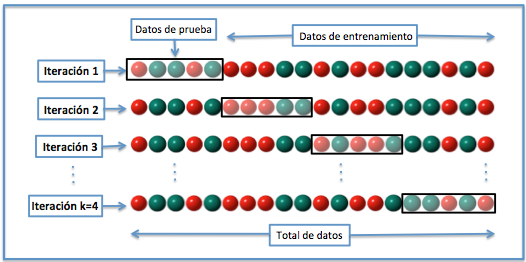
\includegraphics[scale=.5]{validacionCruzada.jpg}
	\caption{Esquema representativo de validación cruzada.}
	\label{VC}
\end{figure}

A modo de ejemplo, sea $K=10$ el número de divisiones a realizar, esto implica, que para un conjunto de datos de tamaño $n$ se forman 10 sub conjuntos de tamaño $n/10$. La validación cruzada implica el entrenamiento y testeo del modelo $K$ veces, en este caso, 10. Por cada iteración, se forma un conjunto de entrenamiento de tamaño $9n/10$ y se testea con un sub conjunto de tamaño $n/10$. 

Por cada iteración, se rota el conjunto de entrenamiento y de testeo, y se obtiene una distribución del desempeño del modelo, reportando el promedio de las métricas asociadas.

\subsubsection{Leave one out}

Es un tipo especial de validación cruzada, en donde se tiene una muestra con $n$ ejemplos en la etapa de entrenamiento se subdivide dicho set de datos considerando $n-1$ elementos, de tal manera que 1 no se considera, la idea en particular radica en entrenar con los $n-1$ ejemplos y validar o testear con el ejemplo restante, esto se itera $n$ veces, tal como se expone en \ref{LOO}, implicando una mayor cantidad de iteraciones que validación cruzada, provocando además un mayor coste computacional \cite{kohavi1995study}.

\begin{figure}[!h]
	\centering
	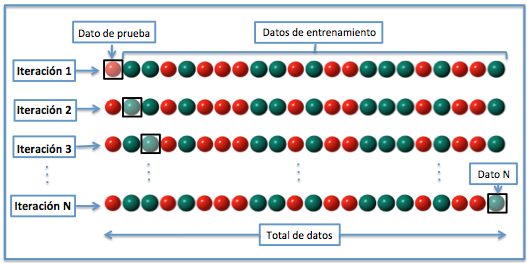
\includegraphics[scale=.5]{Leave-one-out.jpg}
	\caption{Esquema representativo de Leave One.}
	\label{LOO}
\end{figure}

Es decir, es un caso particular de validación cruzada, donde $K=n$ siendo $n$ el número de ejemplos en el conjunto de datos.

Este tipo de validación, provoca disminuciones en las medidas de desempeño, ya que, aumentan la cantidad de puntos en la distribución. Además, en términos computacionales, resulta ser más costosa, por lo que se suele emplear con conjuntos de datos de tamaño bajo, normalmente, menores a 20 ejemplos.

\section{Herramientas computacionales asociadas a evaluación de mutaciones}

Las herramientas computacionales asociadas a la evaluación de mutaciones puntuales se centran principalmente en el análisis de cómo ésta afecta a la estabilidad o la predicción de energía libre asociada a los residuos involucrados en la mutación. Sin embargo, a pesar de que el objetivo es el mismo, se enfocan en diferentes puntos de vista para abordar la problemática, tanto a nivel de entrenamiento de modelos, cómo manipulación de set de datos, así como las técnicas utilizadas para la predicción de los cambios de energía libre.

En la Tabla \ref{tab:tab-summary-tools} se exponen las principales herramientas existentes para la evaluación de la estabilidad de proteínas evaluando mutaciones puntuales, presentando las características, tipos de datos de entrada, resultados, estado de la herramienta y cuáles son las limitantes asociadas

% Please add the following required packages to your document preamble:
% \usepackage{longtable}
% Note: It may be necessary to compile the document several times to get a multi-page table to line up properly
\begin{longtable}[c]{|l|l|l|l|l|}
	\hline
	\multicolumn{1}{|c|}{\textbf{Herr.}}                 & \multicolumn{1}{c|}{\textbf{Características}}                                                                                                                                                                                                                                                                                                                               & \multicolumn{1}{c|}{\textbf{Entradas}}                                                                                                                           & \multicolumn{1}{c|}{\textbf{Salidas}}                                                                                                                                                                                                                         & \multicolumn{1}{c|}{\textbf{Disp.}}                                                  \\ \hline
	\endfirsthead
	%
	\endhead
	%
	Foldx                                                & \begin{tabular}[c]{@{}l@{}}Predice el valor del\\ DDG a través del uso\\ de funciones de energía\\ derivados de términos\\ fisicoquímicos, \\ estadísticos e\\ información estructural\end{tabular}                                                                                                                                                                          & \begin{tabular}[c]{@{}l@{}}Estructura en\\ formato PDB\\ e información\\ sobre la mutación\end{tabular}                                                          & \begin{tabular}[c]{@{}l@{}}Estimación de\\ la diferenciade\\ energía libre\end{tabular}                                                                                                                                                                       & \begin{tabular}[c]{@{}l@{}}Disponible\\ mediante\\ licencia\\ académica\end{tabular} \\ \hline
	I-Mutant                                             & \begin{tabular}[c]{@{}l@{}}Método basado en SVM\\ para la predicción de\\ DDG y la clasificación\\ de la estabilidad de una\\ proteína ante mutaciones\\ puntuales. La mutación es\\ caracterizada a través de\\ propiedades estructurales\\ y la información del\\ ambiente.  Permite la\\ manipulación tanto de\\ secuencias lineales\\ como estructuras PDB\end{tabular} & \begin{tabular}[c]{@{}l@{}}Secuencia lineal\\ proteína, posición\\ y mutación, en\\ caso de existir\\ estructura 3D, se\\ requiere el archivo\\ PDB\end{tabular} & \begin{tabular}[c]{@{}l@{}}Predicción del\\ DDG asociado \\ a la mutación o\\ clasificación\\ de la mutación \\ en estable o\\ desestabilizante\end{tabular}                                                                                                  & \begin{tabular}[c]{@{}l@{}}Disponible\\ para\\ ejecución\\ local\end{tabular}        \\ \hline
	CUPSAT                                               & \begin{tabular}[c]{@{}l@{}}Predice el DDG usando\\ información estructural\\ y del ambiente asociado\\ a la mutación, además\\ utiliza diferentes\\ propiedades estructurales\\ para estimar el valor de\\ energía libre. Este es un\\ método sólo basado en\\ estimaciones utilizando\\ técnicas de\\ bioinformática\\ estructural.\end{tabular}                           & \begin{tabular}[c]{@{}l@{}}Estructura en\\ formato PDB\\ y la posición\\ del residuo a mutar\end{tabular}                                                        & \begin{tabular}[c]{@{}l@{}}Información sobre\\ las 19 posibles\\ sustituciones a\\ realizar, referidas\\ a términos como:\\ ángulos de torsión,\\ accesibilidad\\ al solvente, tipo de\\ estructura\\ secundaria,\\ dentro de las\\ principales.\end{tabular} & No disponible                                                                        \\ \hline
	Dmutant                                              & \begin{tabular}[c]{@{}l@{}}Se basa en el uso de\\ potenciales energéticos\\ para entrenar modelos,\\ utiliza distancias para\\ describir el ambiente y\\ estima el DDG asociado\\ a la mutación\end{tabular}                                                                                                                                                                & \begin{tabular}[c]{@{}l@{}}Estructura en\\ formato PDB\end{tabular}                                                                                              & \begin{tabular}[c]{@{}l@{}}Predicción del\\ DDG asociado\\ a la mutación\end{tabular}                                                                                                                                                                         & No disponible                                                                        \\ \hline
	\begin{tabular}[c]{@{}l@{}}AUTO-\\ MUTE\end{tabular} & \begin{tabular}[c]{@{}l@{}}Manipula las coordenadas\\ de los residuos y aplica\\ triangulación de Delaunay\\ para forma geometrías,\\ así permite describir el\\ ambiente bajo el cual se\\ encuentra el residuo.\\ Los clasificadores se\\ construyen entrenando\\ con Random Forest y\\ los predictores a\\ través de árbolesde\\ decisión.\end{tabular}                  & \begin{tabular}[c]{@{}l@{}}ID-PDB,\\ cadena y\\ mutación\end{tabular}                                                                                            & \begin{tabular}[c]{@{}l@{}}Predicción DDG\\ o clasificación\\ estabilidad,\\ además de\\ información\\ relacionada al\\ sector donde\\ ocurre la\\ mutación\end{tabular}                                                                                      & \begin{tabular}[c]{@{}l@{}}Descargable\\ para\\ ejecución\\ local\end{tabular}       \\ \hline
	\caption{Principales herramientas computacionales enfocadas a la evaluación de la estabilidad o predicción de cambios en la energía libre, asociado a mutaciones puntuales en proteína.
	}
	\label{tab:tab-summary-tools}\\
\end{longtable}

Diferentes son los puntos de vista que pueden ser considerados a la hora de evaluar el efecto que provoca la sustitución de residuos en la estabilidad de una proteína. Ya sea por medio de la estimación utilizando funciones de energía o potenciales energéticos (FoldX \cite{Schymkowitz2005}, Dmutant \cite{Zhou2004}, CUPSAT \cite{Parthiban2006}). Por otro lado, se encuentran métodos basados en algoritmos de apredizaje supervisado. No obstante, estos pueden ser diferenciados con respecto al algoritmo de entrenamiento utilizado o a la forma de describir la mutación. Por ejemplo, I-Mutant \cite{Capriotti2005}, utiliza SVM para predecir o clasificar el efecto de la mutación. Mientras que, AUTO-MUTE \cite{Masso2010} utiliza Random Forest para la clasificación del efecto y Árboles de decisión como algoritmo de regresión.

Cada uno entrega distintas ventajas y desventajas, las cuales se basan principalmente, en la precisión del método y en el tiempo de cómputo relacionado al procedimiento. No obstante, también influye la disponibilidad de estos y si permiten descargas de código fuente para ejecuciones locales o simplemente disponen de versiones web. 


\subsection{Herramientas necesarias para la caracterización de los set de datos}

Adicional a las herramientas expuestas, se hace una descripción breve de SDM \cite{Pandurangan2017} y MOSST \cite{Olivera-Nappa2011}, las cuales serán utilizadas a lo largo de la metodología con el fin de poder caracterizar las mutaciones desde los puntos de vista termodinámico, aplicando SDM y filogenético, por medio de MOSST.

\subsubsection{SDM}

Site Directed Mutator (SDM) \cite{Pandurangan2017}, es una de las herramientas más utilizadas a la hora de evaluar mutaciones puntuales en una proteína de interés y cuyo objetivo principal, es estudiar el efecto sobre la estabiliadd de la proteína que provoca el cambio del residuo.

Se basa en potenciales estadísticos de funciones de energía, para obtener una cuantificación del efecto de una sustitución de un residuo. Este valor se representa por la diferencia de energía libre de Gibbs ($\Delta  \Delta G$). Para estimar el efecto, utiliza ambientes específicos de frecuencias de sustituciones de aminoácidos, sin la utilización de familias de proteínas homólogas. 


Para realizar la estimación, SDM recibe un archivo PDB en el cual se describe la estructura de la proteína inicial, seguido además de la mutación, la cual se describe mediante \textit{"W-Pos-M"}, los cuales corresponden a: Wilde residue, posición en la que se encuentra y mutate residue, respectivamente.

Sus medidas de desempeño en cuanto a la correlación entre los elementos predichos y los reales alcanza un 0.8, calculada a partir del testeo de la herramienta con mutaciones en la proteína Barnasa y staphylococcal nuclease. Este desempeño, lo convierte en una herramienta bastante precisa a la hora de estudiar nuevas predicciones.

Una de las principales razones de utilizar SDM y no otras herramientas computacionales, como las expuestas en la Tabla \ref{tab:tab-summary-tools}, es el hecho de basarse en potenciales estadísticos. Si bien, esta metodología no es tan precisa como el uso de potenciales físicos de funciones de energía, el hecho de utilizar simulaciones basadas en mecanismos de Monte Carlo, conlleva un gran costo computacional en horas de cálculo y recursos. No obstante, es mucho más eficiente que los métodos basados en Machine Learning, dado a que estos, normalmente, tienden a ajustarse y se requiere una gran cantidad de datos para entrenar estos modelos. Además, ya que estos se basan principalmente en métodos asociados a Support Vector Machine (SVM) o Redes Neuronales. Los primeros, no son capaces de adaptarse a espacios altamente no lineales. Mientras que los basados en redes neuronales, no permiten aprender de los atributos empleados, debido a la forma en cómo estos trabajan.

Además, SDM entrega resultados adicionales que permiten comprender el ambiente bajo el cual se produce la mutación y cómo, propiedades termodinámicas se ven afectadas ante la sustitución de residuos.

\subsubsection{MOSST}

Mutagenesis Objetive Search and Selection Tool (MOSST) \cite{Olivera-Nappa2011}, es una herramienta que permite analizar una proteína de interés, con respecto a un conjunto de proteínas con relación filogenética, representadas en un alineamiento múltiple de secuencias. Esto con el fin, de poder detectar posiciones en la proteína de interés o target, que podrían ser mutadas para alterar o no las características de la misma.

Por otro lado , permite estimar mutagénesis relacionadas con la posibilidad de si un cambio de aminoácido dado tendría efectos perjudiciales sobre la proteína. 

Además, como un uso alternativo, es factible la identificación de nsSNPs cuyos fenotipos son relevantes en una familia de genes, permitiendo separar, a aquellas sustituciones que no tienen implicaciones a nivel de funcionalidad.


MOSST aplica técnicas estadísticas para el análisis de las posiciones y se centran en comprender los efectos de las sustituciones desde el punto de vista filogenético. Esto es relevante, ya que como input, sólo necesita secuencias lineales de proteínas, es decir, no es necesario el uso de estructuras en formato PDB, lo cual permite abarcar un mayor número de proteínas de estudio.

Actualmente MOSST se encuentra disponible vía ejecución local, implementado bajo lenguaje de programación Matlab. No obstante, posee una versión online para su uso, facilitando el acceso a la herramienta a diferentes estratos de público.

Utilizar la herramienta MOSST como generación de descriptores basados en propiedades filogenéticas, radica en las ventajas que ésta presenta. Por un lado, permite evaluar la propensión de la mutación y cómo ésta afecta a las características de la proteína en estudio y su familia. Además, permite entender conceptos relacionados a mutaciones, que no son considerados al utilizar propiedades termodinámicas y estructurales. Ya que, estos últimos, sólo evalúan el ambiente bajo el cual ocurre la mutación, mientras que MOSST, evalúa la propensión al cambio. 

El uso de las herramientas MOSST y SDM permitirán describir las mutaciones desde los puntos de vista filogenético y termodinámico-estructural, de tal manera, las falencias de cada método, se complementan, facilitando la generación de descriptores relevantes para las mutaciones.

\section{Hipótesis}

En base a las herramientas existentes y en vista del aumento considerable de datos asociados a mutaciones en proteínas y el conocimiento de las respuestas que éstas generan, se evidencia la necesidad del desarrollo de herramientas computacionales o nuevos modelos de clasificación o regresión que faciliten el entrenamiento de proteínas singulares y la evaluación de sus mutaciones puntuales, con el fin de poder evaluar nuevos ejemplos y cuáles serían los efectos de estos, sin tener que recurrir en grandes costos económicos y tiempos de espera. 

Dado esto se propone la siguiente hipótesis.\\

\textit{El uso de propiedades filogenéticas, termodinámicas y estructurales como descriptores de mutaciones permite el desarrollo de modelos predictivos inspirados en sistemas de meta-learning?}\\

Además de la hipótesis central surgen interrogantes como.

\begin{itemize}
	
	\item Es posible utilizar estos nuevos modelos como herramientas para diagnóstico médico?
	\item Cómo se evalúan la robustez y la generalización de estos modelos, serán capaces de adaptarse a nuevos ejemplos?
	\item Es factible el desarrollo de una herramienta computacional que permita entrenar diferentes set de datos y que facilite la predicción de nuevos ejemplos?
	
\end{itemize}

\section{Objetivos}

En base a la hipótesis planteada y a las preguntas adicionales expuestas, se exponen a continuación el objetivo general y los objetivos específicos.

\subsection{Objetivo general}

Diseñar e implementar estrategias inspiradas en Meta Learning para la implementación de modelos de clasificación y regresión, asociados a mutaciones puntuales en proteínas de interés basados en descriptores termodinámicos, estructurales y filogenéticos.

\subsection{Objetivos específicos}

Dentro de los objetivos específicos se encuentran los siguientes.

\begin{enumerate}
	
	\item Preparar y describir, por medio de propiedades termodinámicas, estructurales y filogenéticas, set de datos de mutaciones puntuales de proteínas con respuesta conocida expuestos en bibliografía o bases de datos públicas.
	
	\item Implementar y evaluar metodología de meta learning para el diseño de meta modelos de clasificación y regresión de mutaciones puntuales aplicados a set de datos de proteínas generadas.
	
	\item Diseñar e implementar herramienta computacional que permita el entrenamiento de set de datos y el uso de meta modelos para la evaluación de nuevos ejemplos.
	
	\item Testear y evaluar comportamiento de la herramienta y los meta modelos en base a sistemas de datos que involucren mutaciones en proteínas con respuesta conocida.
	
	\item Implementar modelos de clasificación para la relevancia clínica de mutaciones puntuales en proteína pVHL, asociada a la enfermedad von Hippel Lindau. 
	
\end{enumerate}

\section{Metodología propuesta}

Con el fin de poder responder a la hipótesis planteada y dar solución a los objetivos impuestos, se propone una metodología general, en la cual, se consideran diferentes estrategias, implementaciones y evaluación de modelos. A continuación se explica la metodología propuesta y los componentes principales de ésta.

\subsection{Preparación de set de datos}

La preparación del set de datos consiste en obtener data para poder entrenar los modelos  predictivos, la data se asocia a información de mutaciones en proteínas y la respuesta que ésta genera. En la Figura \ref{C2:M1} se expone un esquema general con los pasos desarrollados para la preparación del set de datos.

\begin{figure}[!h]
	\centering
	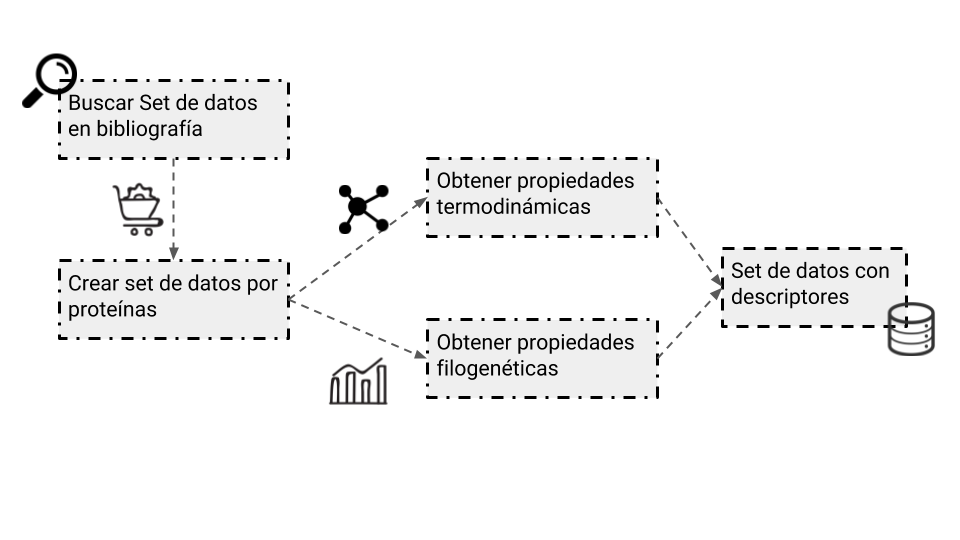
\includegraphics[scale=.4]{m1.png}
	\caption{Esquema representativo asociado al proceso de generación de set de datos de mutaciones puntuales en proteínas.}
	\label{C2:M1}
\end{figure}

Tal como se expone en la Figura \ref{C2:M1}, los set de datos se buscan en la bibliografía, a partir de modelos desarrollados previamente, bases de datos, en la literatura, etc. El objetivo fundamental, es encontrar proteínas con mutaciones puntuales cuyo efecto sea conocido, dicha respuesta puede ser categórica, es decir, asociada al diseño e implementación de modelos de clasificación o continua y se aplica para modelos de regresión. 

En una segunda instancia, a partir de la data recolectada, ésta se procesa con el fin de poder obtener set de datos de proteínas individuales con una cantidad de ejemplos considerables que permitan el diseño de modelos válidos, para ello, fueron implementados scripts bajo el lenguaje de programación Python con el fin de recuperar las proteínas, obtener la información y generar la data de manera individual, además, eliminar ejemplos ambiguos. Es decir, filas con los mismos valores pero cuya columna de respuesta fuese diferente. 

A partir de esto, se forman $n$ set de datos asociados a $n$ proteínas, cada uno con $m$ ejemplos y cuyos descriptores consisten en el residuo original, posición en proteína, residuo mutado y la respuesta asociada. El desbalance de clases se analiza con respecto a las posibles categorías existentes en la respuesta y el porcentaje de representatividad que éstas poseen en la muestra. Se considera que el set de datos exhibe este comportamiento cuando presentan las características expuestas en la sección \ref{problemas}. En el caso de detectar esta problemática, el conjunto de datos será tratado empleando el método SMOTE (Synthetic Minority Oversampling Technique) \cite{chawla2002smote}.

Posteriormente, se aplican las herramientas SDM \cite{Pandurangan2017} y MOSST \cite{Olivera-Nappa2011} con el fin de obtener los descriptores asociados a las propiedades termodinámicas y filogenéticas, respectivamente. Para ello, scripts implementados en lenguaje de programación Python, son desarrollados para consumir los servicios de dichas herramientas y registrar los resultados obtenidos, formando así, set de datos con los descriptores planteados en los objetivos iniciales. Un punto importante a destacar, es que el uso de SDM implica que las proteínas a trabajar, deben presentar una estructura 3D reportada en el Protein Data Bank \cite{berman2000protein} o al menos poseer un modelo representativo y validado. Esto es debido a que se utilizan informaciones de coordenadas para la estimación del efecto de la mutación, minimizaciones energéticas y estabilización de la mutante.

Ya con los descriptores formados, las características asociadas a variables categóricas son codificadas. Si la totalidad de posibles categorías supera el 20\% del total de características en el set de datos, se aplica Ordinal Encoder, en caso contrario, One Hot Encoder \cite{pedregosa2011scikit}. Ordinal Encoder consiste en la transformación de variables categóricas en arreglos de números enteros con valores desde $0,...,n-1$ para $n$ posibles categorías. Por otro lado, One Hot Encoder, consiste en agregar tantas columnas como posibles categorías existan en el set de datos completadas mediante binarización de elementos (0 si la característica no se presencia, 1 en caso contrario)\footnote{Más detalles sobre la codificación de variables categóricas y secuencias lineales de proteínas serán tratadas en el capítulo \ref{cap3}.}.

Es importante mencionar, que las respuestas asociadas a las mutaciones pueden ser del tipo continuo o categórico, lo cual implica que tanto los modelos como las métricas varían. No obstante, se aplica la metodología indistintamente, con el fin de demostrar la robustez del método y la eficacia de éste sin importar el tipo de modelo que se éste entrenando.

\subsection{Implementación de meta modelos de clasificación/regresión}

La implementación de meta modelos consiste en la obtención de un grupo de estimadores que en conjunto, permiten clasificar o predecir nuevos ejemplos. Para ello, se diseña e implementa una metodología inspirada en Sistemas de Meta Learning y aplicando técnicas estadísticas para la evaluación del desempeño y el uso del meta modelo con nuevos ejemplos.

En la Figura \ref{C2:M2}, se exponen las etapas asociadas a la implementación de meta modelos, contemplando desde la fase de entrenamiento de los modelos hasta la unión en meta clasificadores, lo cual se reporta en la herramienta MLSTools (Paper en redacción). 

Cada una de las etapas, contempla un conjunto de scripts implementados en lenguaje de programación Python y empleando la librería Scikit-Learn para el entrenamiento y evaluación de los clasificadores o predictores \cite{pedregosa2011scikit}, así como Numpy para el uso de módulos estadísticos \cite{doi:10.1109/MCSE.2011.37}.


\begin{figure}[!h]
	\centering
	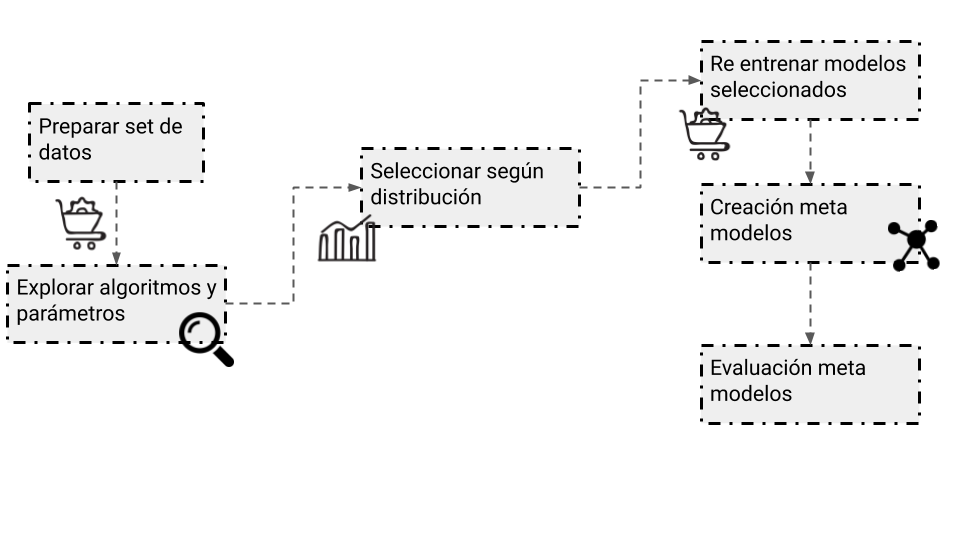
\includegraphics[scale=.4]{m2.png}
	\caption{Esquema representativo asociado al proceso de creación de meta modelos utilizando la metodología reportada para la herramienta MLSTools (Paper en redacción).}
	\label{C2:M2}
\end{figure}

Tal como se observa en la Figura \ref{C2:M2}, es posible identificar etapas claves en el proceso: Exploración de modelos, Selección y Generación de los meta clasificadores/predictores, junto con su evaluación. Cada una de estas etapas se exponen a continuación.

\subsubsection{Exploración de modelos}

La exploración de modelos o estimadores, se basa en la aplicación de diferentes algoritmos de aprendizaje supervisado con variaciones en sus parámetros de configuración inicial. La utilización de los algoritmos, depende principalmente del tipo de respuesta que presente el set de datos, es decir, si es continua o categórica. No obstante, a modo resumen, en la Tabla \ref{cap2:tab1} se exponen los algoritmos utilizados, el caso en el que se usan y los parámetros que se varían junto con el total de iteraciones posibles para cada elemento:

\begin{longtable}[c]{llll|l|l|}
	\hline
	\multicolumn{6}{|c|}{\textbf{Algoritmos y parámetros empleados en la etapa de Exploración en MLSTools}}                                                                                                                                                                                                                                                                                               \\ \hline
	\endfirsthead
	%
	\endhead
	%
	\multicolumn{1}{|l|}{\textbf{\#}} & \multicolumn{1}{l|}{\textbf{Algoritmo}}                                                  & \multicolumn{1}{l|}{\textbf{Tipo}}    & \textbf{Parámetros}                                                                                                                 & \textbf{Uso}                                                         & \textbf{Iteraciones} \\ \hline
	\multicolumn{1}{|l|}{1.}          & \multicolumn{1}{l|}{Adaboost}                                                            & \multicolumn{1}{l|}{Ensamble}         & \begin{tabular}[c]{@{}l@{}}Algoritmo\\ Número estimadores\end{tabular}                                                              & \begin{tabular}[c]{@{}l@{}}Clasificación \\ y Regresión\end{tabular} & 16                   \\ \hline
	\multicolumn{1}{|l|}{2.}          & \multicolumn{1}{l|}{Bagging}                                                             & \multicolumn{1}{l|}{Ensamble}         & \begin{tabular}[c]{@{}l@{}}Bootstrap\\ Número estimadores\end{tabular}                                                              & \begin{tabular}[c]{@{}l@{}}Clasificación y\\ Regresión\end{tabular}  & 16                   \\ \hline
	\multicolumn{1}{|l|}{3.}          & \multicolumn{1}{l|}{\begin{tabular}[c]{@{}l@{}}Bernoulli\\ Naive Bayes\end{tabular}}     & \multicolumn{1}{l|}{Probabilístico}   & Default                                                                                                                             & Clasificación                                                        & 1                    \\ \hline
	\multicolumn{1}{|l|}{4.}          & \multicolumn{1}{l|}{Decision Tree}                                                       & \multicolumn{1}{l|}{Características}  & \begin{tabular}[c]{@{}l@{}}Criterio división\\ Función de impureza\end{tabular}                                                     & \begin{tabular}[c]{@{}l@{}}Clasificación y\\ Regresión\end{tabular}  & 4                    \\ \hline
	\multicolumn{1}{|l|}{5.}          & \multicolumn{1}{l|}{\begin{tabular}[c]{@{}l@{}}Gaussian\\ Naive Bayes\end{tabular}}      & \multicolumn{1}{l|}{Ensamble}         & Default                                                                                                                             & \begin{tabular}[c]{@{}l@{}}Clasificación y\\ Regresión\end{tabular}  & 1                    \\ \hline
	\multicolumn{1}{|l|}{6.}          & \multicolumn{1}{l|}{\begin{tabular}[c]{@{}l@{}}Gradient\\ Tree Boosting\end{tabular}}    & \multicolumn{1}{l|}{Ensamble}         & \begin{tabular}[c]{@{}l@{}}Función de pérdida\\ Número estimadores\end{tabular}                                                     & \begin{tabular}[c]{@{}l@{}}Clasificación y\\ Regresión\end{tabular}  & 16                   \\ \hline
	\multicolumn{1}{|l|}{7.}          & \multicolumn{1}{l|}{\begin{tabular}[c]{@{}l@{}}k-Nearest\\ Neighbors\end{tabular}}       & \multicolumn{1}{l|}{Distancias}       & \begin{tabular}[c]{@{}l@{}}Número Vecinos\\ Algoritmo\\ Métrica distanciaPesos\end{tabular}                                         & \begin{tabular}[c]{@{}l@{}}Clasificación y\\ Regresión\end{tabular}  & 160                  \\ \hline
	\multicolumn{1}{|l|}{9.}          & \multicolumn{1}{l|}{\begin{tabular}[c]{@{}l@{}}Nu Support\\ Vector Machine\end{tabular}} & \multicolumn{1}{l|}{Kernel}           & \begin{tabular}[c]{@{}l@{}}Kernel\\ Nu\\ Grado polinomio\end{tabular}                                                               & \begin{tabular}[c]{@{}l@{}}Clasificación y\\ Regresión\end{tabular}  & 240                  \\ \hline
	\multicolumn{1}{|l|}{10.}         & \multicolumn{1}{l|}{Random Forest}                                                       & \multicolumn{1}{l|}{Ensamble}         & \begin{tabular}[c]{@{}l@{}}Número estimadores\\ Función de impureza\\ Bootstrap\end{tabular}                                        & \begin{tabular}[c]{@{}l@{}}Clasificación y\\ Regresión\end{tabular}  & 32                   \\ \hline
	\multicolumn{1}{|l|}{11.}         & \multicolumn{1}{l|}{\begin{tabular}[c]{@{}l@{}}Support\\ Vector Machine\end{tabular}}    & \multicolumn{1}{l|}{Kernel}           & \begin{tabular}[c]{@{}l@{}}Kernel\\ C\\ Grado polinómio\end{tabular}                                                                & \begin{tabular}[c]{@{}l@{}}Clasificación y\\ Regresión\end{tabular}  & 240                  \\ \hline
	&                                                                                          &                                       &                                                                                                                                     & \textbf{Total Iteraciones}                                           & \textbf{726}        \\ \cline{5-6} 
	\caption{Tabla resumen, algoritmos implementados, parámetros utilizados e iteraciones involucradas por cada algoritmo.}
	\label{cap2:tab1}\\
\end{longtable}

Como se observa en la Tabla \ref{cap2:tab1}, son sobre 720 modelos los que se generan y a partir de ellos se obtiene distribuciones de medidas de desempeño que permiten evaluarlos. En el caso de modelos de regresión se utilizan los coeficientes de Pearson, Spearman, Kendall $\tau$ y $R^{2}$, mientras que para modelos de clasificación, se consideran la Precisión, Exactitud, Recall y F1.

Finalmente, esta etapa, entrega set de modelos entrenados y evaluados según las métricas de interés. Se destaca que cada modelo es validado a través del proceso de validación cruzada, con el fin de poder disminuir posibles sobreajustes. El valor de $k$ asociado a las subdivisiones a realizar varía con respecto a la cantidad de ejemplos que presente el set de datos, es decir, sea $n$ la cantidad de ejemplos en la muestra, si $n<=20$ se tiene que $k=n$ implicando el uso de Leave one out, si $n>20$ y $n<=50$ se considera un valor de $k=3$, si $n>50$ y $n<=100$ $k=5$, por último, si $n>100$ se tiene un valor de $k=10$.

\subsubsection{Selección de modelos}

Cada distribución de medida de desempeño perteneciente a los modelos entrenados en la fase de Exploración, se somete a test estadísticos basados en Z-score \cite{pedregosa2011scikit} que permite seleccionar los modelos cuyas métricas representen outliers positivos dentro de la distribución.

El algoritmo general, utilizado para el desarrollo de esta selección es como se expone en el algoritmo \ref{alg:select}, para el cual se detallan los pasos simplificados que permiten obtener un conjunto de modelos entrenados y que representan los valores más altos dentro de su distribución. Es importante mencionar, que se obtiene un conjunto $M'$ con los modelos, considerando como punto de selecciones los valores evaluados con respecto a la desviación estándar, considerando los umbrales 3 $\sigma$, 2 $\sigma$ y 1.5 $\sigma$ por sobre la media, si ningún factor se cumple, sólo se considera el valor máximo en la distribución.

Es importante mencionar, que cada distribución puede permitir la selección de distintos modelos, lo cual implica que un mismo modelo pueda ser seleccionado en diferentes medidas, razón por la cual, a la hora de obtener el conjunto de modelos $M'$ se remueven aquellos elementos que se encuentran repetidos. Siendo estos, sólo los modelos que presenten igualdad tanto en el algoritmo como en sus parámetros de configuración inicial.

\begin{algorithm}[H]
	\begin{algorithmic}[1]
		\REQUIRE Conjunto $M$ con modelos entrenados y sus medidas de desempeño, Lista $L$ con medidas de desempeño. \label{lin:lineaRara}
		\ENSURE Conjunto $M'$ con modelos seleccionados.
		
		
		\FOR{$i$ en $L$} 
		\STATE Calcular  media $\mu$, desviación estándar $\sigma$ en distribución $M_{i}$
		\FOR{$ x \in M_{i}$}
		\IF {$x \ge \mu + 3*\sigma$}
		\STATE Agregar $x$ a $M'$
		\ENDIF
		\ENDFOR
		\IF {largo $M'$ = 0}
		\FOR{$ x \in M_{i}$}
		\IF {$x \ge \mu + 2*\sigma$}
		\STATE Agregar $x$ a $M'$
		\ENDIF
		\ENDFOR
		
		\IF {largo $M'$ = 0}
		\FOR{$ x \in M_{i}$}
		\IF {$x \ge \mu + 1.5*\sigma$}
		\STATE Agregar $x$ a $M'$
		\ENDIF
		\ENDFOR
		
		\IF {largo $M'$ = 0}
		\FOR{$ x \in M_{i}$}
		\IF {$x = MAX{M_{i}}$}
		\STATE Agregar $x$ a $M'$
		\ENDIF
		\ENDFOR
		\ENDIF
		\ENDIF
		\ENDIF
		\ENDFOR
		
		\RETURN $D$ sin valores extremos
	\end{algorithmic}
	\caption{Algoritmo de selección de modelos}\label{alg:select}
\end{algorithm}

\subsubsection{Generación y evaluación de meta modelos}

A partir del conjunto de modelos $M'$, el cual representa los estimadores seleccionados, cuyas medidas de desempeño son las más altas en sus distribuciones correspondientes, se generan meta modelos, es decir, estimadores compuestos de diversas unidades, los cuales en conjunto entregan una respuesta, ya sea por ponderación o votación. El proceso general para la generación de los meta modelos, es descrito a continuación.

En una primera instancia, los modelos son nuevamente entrenados y se comparan las nuevas medidas de desempeño con las obtenidas previamente. En caso de que exista una diferencia mayor al 20\%, en cualquiera de sus métricas, el modelo se remueve del conjunto $M'$. La razón fundamental de esto, es debido a que se espera desarrollar modelos robustos cuyas evaluaciones no presenten variaciones significativas y que realmente no alteren sus predicciones ante nuevos ejemplos, razón por la cual, se aplica nuevamente validación cruzada para validar los modelos.

Con el fin de evaluar el desempeño de los meta modelos, nuevas medidas se generan a partir de la información resultante de los modelos individuales. No obstante, la forma en la que se obtienen varían dependiendo del tipo de respuesta que se debe entregar.

Si la respuesta es continua, se obtiene los valores de predicción de cada modelo y se promedian, para luego aplicar las métricas estándar (Coeficiente de Pearson, Kendall $\tau$, Spearman y $R^{2}$) sobre estos valores promediados y los reales. Expresado matemáticamente:

Sea $M'$ la cantidad de elementos en el meta modelo, $n$ la cantidad de ejemplos en el set de datos y sea $Y$ el vector de respuestas reales de tamaño $n$. Para cada $M'_{i}\ \in\ M'$ se obtiene un vector $Y_{i}$ que representa los valores de predicción entregados por el modelo $M'_{i}$. A partir de cada $Y_{i}$ se genera una matriz de predicciones $P(mxn)$ donde $m$ representa la cantidad de modelos en $M'$. Finalmente, se obtiene un vector $Y'$ de tamaño $n$, el cual se compone de la media de cada columna en la matriz $P$, es decir, para el ejemplo $i$ se obtienen $m$ predicciones, las cuales son promediadas, formando el valor $Y'_{i}\ \in\  Y'$. Vector el cual, se utiliza para obtener las métricas de desempeño.

Para el caso en que la respuesta sea categórica, es decir, los modelos son del tipo clasificación, se obtiene la respuesta de cada modelo individual y se selecciona una única categoría, correspondiente a aquella que presente una mayor probabilidad de ocurrencia dada la distribución de elementos y considerando para ello las probabilidades iniciales de cada categoría en el set de datos de estudio. De esta forma, se obtiene un vector respuesta con la clasificación de cada ejemplo cuyo valor corresponde al evento más probable a ocurrir, este vector se compara con el set de respuestas reales y se aplican las métricas de interés para clasificadores.

\subsection{Cómo usar los meta modelos para la clasificación de nuevos ejemplos?}

Nuevos ejemplos pueden ser clasificados o predecir su respuesta, dependiendo sea el caso, a partir de los meta modelos desarrollados. En el caso de estimadores basados en variables continuas, los nuevos ejemplos se someten a cada uno de los modelos individuales pertenecientes al sistema, los cuales generan una respuesta individual, a partir de dichas respuestas, se genera un intervalo de confianza con un nivel de significancia $\alpha=0.01$ donde existe una mayor probabilidad de que se encuentre el valor real de la predicción dado los valores del entrenamiento. Para ejemplos que impliquen clasificación, se obtiene la respuesta de cada modelo individual y se evalúa la probabilidad de ocurrencia de cada categoría, entregando así, la respuesta condicionada por una probabilidad de ocurrencia del evento.

\subsection{Uso de meta modelos en sistemas de proteínas}

El objetivo principal de esta metodología, radica en el hecho de crear una herramienta que permita implementar modelos basados en algoritmos de aprendizaje supervisado para set de datos de mutaciones puntuales o variantes para una misma proteína. 

Un flujo general del uso de la herramienta, se expone en la Figura \ref{C2:M3}.

\begin{figure}[!h]
	\centering
	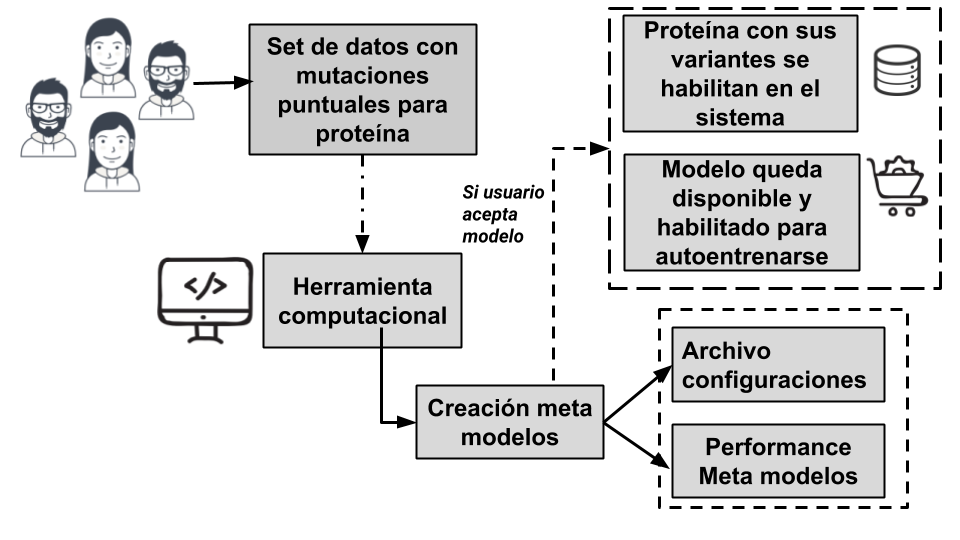
\includegraphics[scale=.4]{m3.png}
	\caption{Esquema representativo de flujo asociado a la herramienta de generación de meta modelos para mutaciones puntuales en proteínas de interés.}
	\label{C2:M3}
\end{figure}

La idea general, consiste en que usuarios de la herramienta, puedan entrenar sus propios modelos de clasificación o regresión, basados en la metodología expuesta en los pasos anteriores mediante el uso de Meta Learning Sytem Tools (Paper en Redacción). Para ello, los usuarios deben entregar sus set de datos con la información necesaria para ser procesada: cadena, residuo original, posición, residuo mutado y respuesta o efecto de la mutación, además del archivo PDB a ser procesado. 

La herramienta, aplica los pasos expuestos en la metodología de este capítulo generando un meta modelo basado en algoritmos de aprendizaje supervisado y las medidas de desempeño que permiten evaluar el modelo obtenido. 

Si el usuario acepta la metodología y permite la publicación de los datos, el sistema habilita el acceso tanto a los meta modelos como a los set de datos y los agrega a la lista de procesos de modelos auto entrenables.

Esto último, implica que ante la adición de nuevos ejemplos al set de datos, el sistema actualiza los modelos y las medidas de desempeño, aplicando la metodología expuesta, así, constantemente mantiene la actualización de la información y permite mantener en constante crecimiento los datos que contemplan el desarrollo de los modelos.

\section{Análisis y evaluación de los set de datos a utilizar}

A continuación, se exponen los resultados obtenidos hasta el momento, presentando principalmente, los set de datos a utilizar, las características que estos poseen y qué representan, con el fin de contextualizar la data a manipular y los modelos a generar.

\subsection{Set de datos utilizados}

En el presente apartado se describen las características básicas de los set de datos trabajados, así como también, qué representan las proteínas bajo las cuales se están desarrollando los modelos de estimadores.

\subsubsection{Descripción general}

Los set de datos utilizados, tanto para la formación de los inputs asociados al sistema, así como también la validación de respuesta correspondiente a la mutación que estos tienen, fueron extraídos desde distintas bases de datos de mutaciones en proteínas de estudios relacionados a los cambios que provoca la sustitución del residuo inicial, ya sea a nivel de cambios energéticos o estabilidad de la proteína.

11 set de datos con respuesta continua fueron obtenidos. Cada set de datos contemplaba como elemento a predecir, las diferencias de energía libre de Gibbs, entre los residuos originales y mutados. Las mutaciones fueron seleccionadas desdes diversos estudios en los cuales se reportaron, centrándose en \cite{Wainreb2011, Sun2017, petukh2016saambe, Alexov2012,prot20185}.

Adicional a los set de datos con respuesta continua, 8 conjuntos de elementos asociados a tareas de clasificación fueron obtenidos desde diversos estudios reportados a la actualidad \cite{ancien2018prediction, broom2017computational, capriotti2008three, quan2016strum, Capriotti2005, 1gzp030, Khan2010, masso2008accurate, getov2016saafec}. 

De tal manera, se generó un total de 19 conjuntos de set de datos, con respuesta categórica y continua, los cuales se asocian a proteínas independientes, usadas para la evaluación de las metodologías planteadas. Estas 19 proteínas junto con su descripción, se exponen en la Tabla \ref{cap2:tab2}.


\begin{longtable}[c]{|l|l|l|l|l|}
	\hline
	\multicolumn{5}{|c|}{\textbf{Resumen set de datos de proteínas y sus características}}                                                                                                                                                                                             \\ \hline
	\endfirsthead
	%
	\endhead
	%
	\textbf{\#} & \textbf{Código PDB} & \textbf{Tipo} & \textbf{Ejemplos} & \textbf{Descripción}                                                                                                                                                                                       \\ \hline
	1.          & 1A22                & Regresión     & 132               & \begin{tabular}[c]{@{}l@{}}Human growth hormone bound to single\\ receptor\end{tabular}                                                                                                                    \\ \hline
	2.          & 1CH0                & Regresión     & 191               & \begin{tabular}[c]{@{}l@{}}Crystal and molecular structures of the complex\\ of alpha-*Chymotrypsin with its inhibitor Turkey\\ Ovomucoid third domain\end{tabular}                                        \\ \hline
	3.          & 1DKT                & Regresión     & 119               & \begin{tabular}[c]{@{}l@{}}CKSHS1: Human cyclin dependent\\ kinase subunit, type 1 complex with\\ metavanadate\end{tabular}                                                                                \\ \hline
	4.          & 1FKJ                & Regresión     & 219               & \begin{tabular}[c]{@{}l@{}}Atomic structure of FKBP12-FK506, \\ an immunophilin  immunosupressant\\ complex\end{tabular}                                                                                   \\ \hline
	5.          & 1FTG                & Regresión     & 203               & \begin{tabular}[c]{@{}l@{}}Structure of apoflavodoxin: closure of\\ a Tyr/Trp aromatic gate leads to a\\ compact fold\end{tabular}                                                                         \\ \hline
	6.          & 1PPF                & Regresión     & 190               & \begin{tabular}[c]{@{}l@{}}X-Ray crystal structure of the complex\\ of human leukocyte elastase and the\\ third domain of the Turkey ovomucoid\\ inhibitor\end{tabular}                                    \\ \hline
	7.          & 1RX4                & Regresión     & 556               & \begin{tabular}[c]{@{}l@{}}Dihydrofolate reductase (E.C.1.5.1.3) complexed\\ with 5,10-Dideazatetrahydrofolate and\\ 2'-Monophosphadenosine 5'-Diphosphoribose\end{tabular}                                \\ \hline
	8.          & 1WQ5                & Regresión     & 239               & \begin{tabular}[c]{@{}l@{}}Crystal structure of tryptophan synthase\\ alpha-subunit from Escherichia coli\end{tabular}                                                                                     \\ \hline
	9.          & 2AFG                & Regresión     & 134               & Human acidic fibroblast growth factor                                                                                                                                                                      \\ \hline
	10.         & 3SGB                & Regresión     & 191               & \begin{tabular}[c]{@{}l@{}}Structure of the complex of Streptomyces\\ Griseus protease B and the Third domain\\ of the Turkey ovomucoid inhibitor\end{tabular}                                             \\ \hline
	11.         & 5AZU                & Regresión     & 203               & \begin{tabular}[c]{@{}l@{}}Crystal structure analysis of oxidize\\ Pseudomonas Aeruginoa Azurin at PH 5.5\\ and PH 9.0. A PH-induced conformational\\ Transition involves a peptide bond flip\end{tabular} \\ \hline
	12.         & 1BN1                & Clasificación & 1802              & Carbonic anhydrase II inhibitor                                                                                                                                                                            \\ \hline
	13.         & 1BVC                & Clasificación & 561               & \begin{tabular}[c]{@{}l@{}}Structure of a Biliverdin Apomyoglobin\\ complex\end{tabular}                                                                                                                   \\ \hline
	14.         & 1LZ1                & Clasificación & 848               & \begin{tabular}[c]{@{}l@{}}Human Lysozyme. Analysis of Non-Bonded\\ and Hydrogen-Bond interactions\end{tabular}                                                                                            \\ \hline
	15.         & 1STN                & Clasificación & 2193              & \begin{tabular}[c]{@{}l@{}}The crystal structure of Staphylococcal\\ Nuclease\end{tabular}                                                                                                                 \\ \hline
	16.         & 1VQB                & Clasificación & 820              & \begin{tabular}[c]{@{}l@{}}Gene V Protein (Single-Stranded DNA\\ Binding Protein)\end{tabular}                                                                                                             \\ \hline
	17.         & 2CI2                & Clasificación & 741               & \begin{tabular}[c]{@{}l@{}}Crystal and molecular structure of the\\ Serine proteinase inhibitor CI-2 from\\ Barley seeds\end{tabular}                                                                      \\ \hline
	18.         & 2LZM                & Clasificación & 2336              & Structure of Baceriophage T4 Lysosyme                                                                                                                                                                      \\ \hline
	19.         & 2RN2                & Clasificación & 712               & \begin{tabular}[c]{@{}l@{}}Structural details of ribonuclease H from\\ Escherichia Coli\end{tabular}                                                                                                       \\ \hline
	\caption{Resumen de proteínas utilizadas para el desarrollo de meta modelos basados en metodología Meta Learning System propuesta durante este capítulo.}
	\label{cap2:tab2}\\
\end{longtable}

Cada una de las proteínas presentan diferentes características y funcionalidades, algunas facilitan la unión a DNA, mientras que otras presentan propiedades enzimáticas, por otro lado, existen enzimas que representan inhibidores, entre las principales. Esto es interesante a la hora de evaluar el poder que presenta la metodología con respecto al análisis de diferentes proteínas, estructuras y complejos, ya que se presenta una gran variedad en cuanto a forma y funcionalidad de éstas, lo que implica que el sistema no se limita por cierto tipo de estructuras o complejos.

A modo de ilustrar las diferencias estructurales de las proteínas en estudio, en la Figura \ref{fig:proteins} se exponen algunas de las estructuras asociadas a las proteínas utilizadas para desarrollar modelos de clasificación o regresión.

\begin{figure}
	\centering
	\begin{subfigure}{0.4\textwidth}
		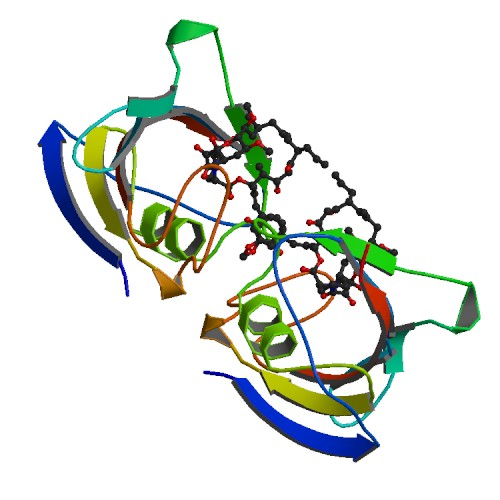
\includegraphics[width=\textwidth]{1fkj.jpg}
		\caption{1FKJ}
		\label{fig:1FKJ}
	\end{subfigure}
	~ %add desired spacing between images, e. g. ~, \quad, \qquad, \hfill etc. 
	%(or a blank line to force the subfigure onto a new line)
	\begin{subfigure}{0.4\textwidth}
		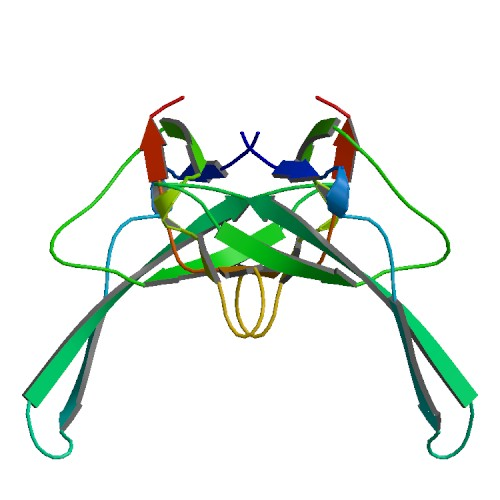
\includegraphics[width=\textwidth]{1vqb.jpg}
		\caption{1VQB}
		\label{fig:1VQB}
	\end{subfigure}
	~ %add desired spacing between images, e. g. ~, \quad, \qquad, \hfill etc. 
	%(or a blank line to force the subfigure onto a new line)
	\begin{subfigure}{0.4\textwidth}
		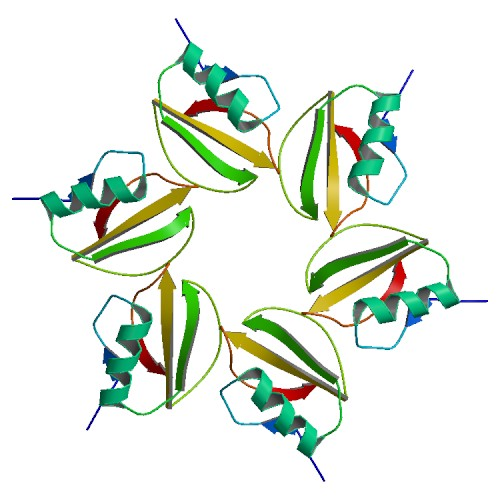
\includegraphics[width=\textwidth]{2ci2.jpg}
		\caption{2CI2}
		\label{fig:2CI2}
	\end{subfigure}
	
	\begin{subfigure}{0.4\textwidth}
		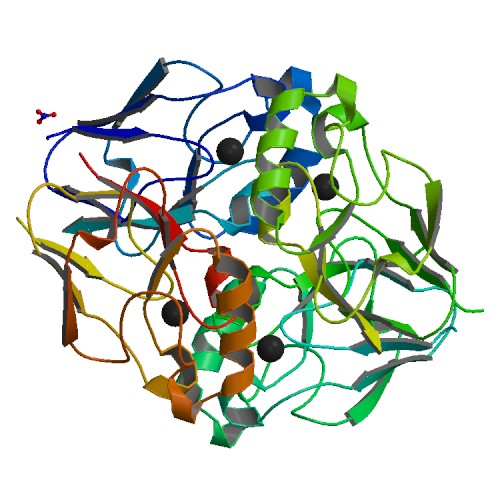
\includegraphics[width=\textwidth]{5azu.jpg}
		\caption{5AZU}
		\label{fig:5AZU}
	\end{subfigure}
	\caption{Representación de estructuras de proteínas ejemplos utilizadas para el desarrollo de meta modelos de clasificación.}
	\label{fig:proteins}
\end{figure}

Las mutaciones fueron recolectadas desde diferentes set de datos, por lo que, en caso de información ambigua, es decir, una misma mutación con diferentes respuestas, no fueron consideradas. Por otro lado, debido a que para la aplicación de la herramienta SDM se necesitaba la cadena a la cual pertenece en residuo, scripts desarrollados en Python y utilizando la librería BioPython, permitieron procesar los archivos asociados a las estructuras de las proteínas, identificadas desde el Protein Data Bank (PDB) \cite{abola1984protein}. Descartando aquellas mutaciones reportadas en las que no se encontró la cadena, obteniendo como resultante la cantidad de mutaciones reportadas para cada proteína expuestas en la Tabla \ref{cap2:tab2}.

\subsubsection{Evaluación del desbalance de clases y distribución de respuestas continuas}

El desbalance de clases se evaluó en aquellos set de datos con respuesta categórica, lo cual contempla, tres posibles casos: Neutral, Estable, No Estable, esto es debido a que todos los estudios donde se evalúan mutaciones, normalmente se analizan cambios que alteren la estabilidad de la proteína. En la Figura \ref{fig:desbalance}, se aprecia a modo ejemplo dos set datos y su distribución de categorías para la variable respuesta.

\begin{figure}[!h]
	\centering
	\begin{subfigure}{0.8\textwidth}
		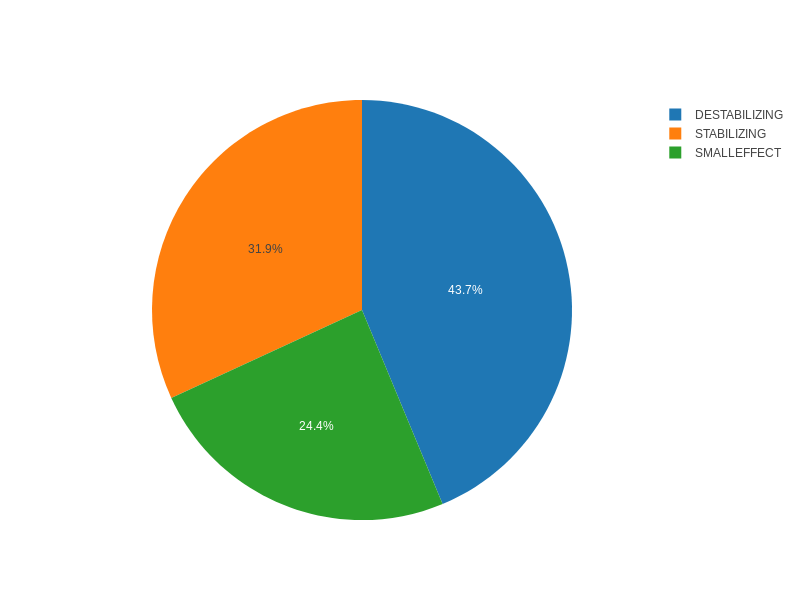
\includegraphics[width=\textwidth]{class1STN.png}
		\caption{1STN}
		\label{fig:des1}
	\end{subfigure}
	~ %add desired spacing between images, e. g. ~, \quad, \qquad, \hfill etc. 
	%(or a blank line to force the subfigure onto a new line)
	\begin{subfigure}{0.8\textwidth}
		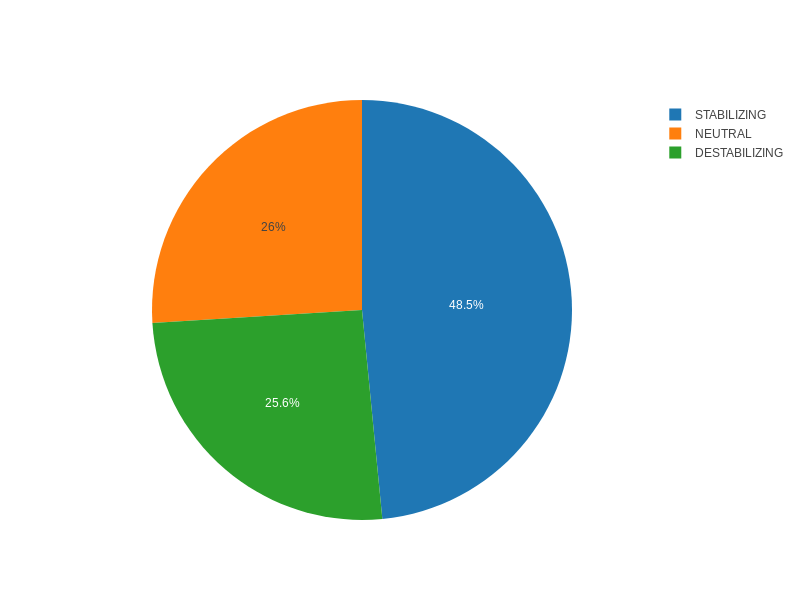
\includegraphics[width=\textwidth]{class2RN2.png}
		\caption{2RN2}
		\label{fig:des2}
	\end{subfigure}
	
	\caption{Evaluación del desbalance de clases en proteínas ejemplo.}
	\label{fig:desbalance}
\end{figure}

En las 8 proteínas en estudio para modelos de clasificación, la distribución de las categorías es similar a lo expuesta en la Figura \ref{fig:desbalance} para todas ellas, donde cerca del 50\% corresponden a mutaciones que afectan positivamente a la estabilidad, mientras que mutaciones que provocan cambios negativos o no generan diferencias, se encuentran en proporciones similares, ambas cercanas al 25\%. 

Si bien las proporciones son dispares, para este caso, se considera un desbalance como un elemento que representa menos de un 5\% del total de la muestra, además, dado a que la cantidad de ejemplos son elevadas, un 20\% o un 25\% implica cerca de 200 mutaciones, en promedio, que cumplen dicha característica. También, el hecho de que exista una cantidad inferior de mutaciones no benéficas a la estabilidad viene dada a la dificultad de encontrar y reportar mutaciones que afecten negativamente a para una proteína, es debido a la propensión filogenética \cite{Olivera-Nappa2011} que estos ocurran, lo cual se ve reflejado en las diferencias asociadas a cambios positivos dentro del set de mutaciones. No obstante, si bien el hecho de que la propensión filogenética indique que el cambio tiende a mejorar estabilidad, diseñar mutantes con mejoras en propiedades de interés, es un problema latente en la actualidad, de alto costo económico y computacional y con una gran demanda desde diferentes áreas del conocimiento.

En los set de datos para el desarrollo de modelos de regresión, se evaluó la distribución de la respuesta, en este caso, valores de $\Delta\Delta\ G$ asociado a diferencias de energía libre producidas entre el residuo mutado y el original, tal que: $\Delta\ Res_{mut}\ - \Delta\ Res_{wild}\ = \Delta\Delta\ G$. 

Las distribuciones se evaluaron utilizando el test de Shapiro, con el fin de determinar si la distribución se comportaba como una normal. Para todas las proteínas estudiadas, en los 11 set de datos, las respuestas presentaron distribución normal, con valores de Shapiro sobre 0.8 y un p-value $\leq$ 0.01, lo cual indica una alta confianza estadística en los resultados presentados por dicho test.

Una visualización de las distribuciones puede generarse a partir del desarrollo de histogramas, los cuales, a modo de ejemplo se expone en la Figura \ref{fig:histogram}.

\begin{figure}[!h]
	\centering
	\begin{subfigure}{0.48\textwidth}
		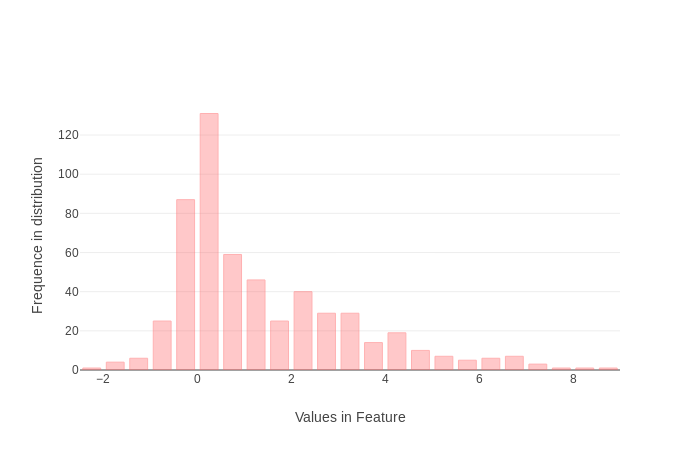
\includegraphics[width=\textwidth]{1RX4.png}
		\caption{Histograma para respuesta continua en 1RX4}
		\label{fig:hist1}
	\end{subfigure}
	~ %add desired spacing between images, e. g. ~, \quad, \qquad, \hfill etc. 
	%(or a blank line to force the subfigure onto a new line)
	\begin{subfigure}{0.48\textwidth}
		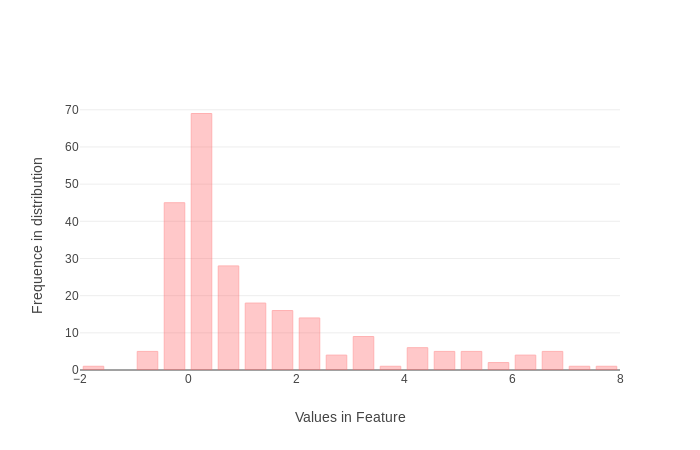
\includegraphics[width=\textwidth]{1WQ5.png}
		\caption{Histograma para respuesta continua en 1WQ5}
		\label{fig:hist2}
	\end{subfigure}
	
	\caption{Evaluación de la distribución de respuesta continua en set de datos de proteínas.}
	\label{fig:histogram}
\end{figure}

El análisis de estas características es relevante a la hora de diseñar modelos de clasificación o regresión, debido a que si existe una tendencia por una clase condiciona al clasificador a \textit{"aprender en base a la mayoría"}, por lo que puede aumentar los errores en cuanto a falsos positivos, dado a que, no se tiene la cantidad de ejemplos suficientes para una clase que permitan al modelo capturar las posibles variaciones asociadas a ésta.

Dado a los análisis de evaluación de representatividad de categorías en el set de datos y distribución de respuestas continuas, se expone que los set de datos seleccionados no presentan desbalance significativo para el caso de desarrollo de modelos de clasificación y a su vez, todas las respuestas asociadas a cambios en la energía libre para modelos de regresión, presentan distribución normal. Razón por la cual, es factible el desarrollo de modelos asociados a las respuestas presenten en los set de datos seleccionados. No obstante, sólo se ha considerado el problema del desbalance y la evaluación de distribución en la respuesta continua, una vez caracterizado los set de datos a partir de las propiedades fisicoquímicas y termodinámicas, se analizarán las características y cómo éstas condicionan la clasificación o la predicción de cambios energéticos.
